% !TeX spellcheck = pl_PL

\newpage
\begin{center}
	{\LARGE \textbf{k - 1000, K - 1024 !!!}}
\end{center}

\part{Zadania}
% ==================================================
% --- 1. TOPOLOGIA SIECI
% ==================================================
\section{Topologia sieci}
	% ================= ZADANIE 1.1 ==================
	\subsection{Zadanie}
		\subsubsection{Treść}
			\begin{wrapfigure}{l}{6.0cm}
				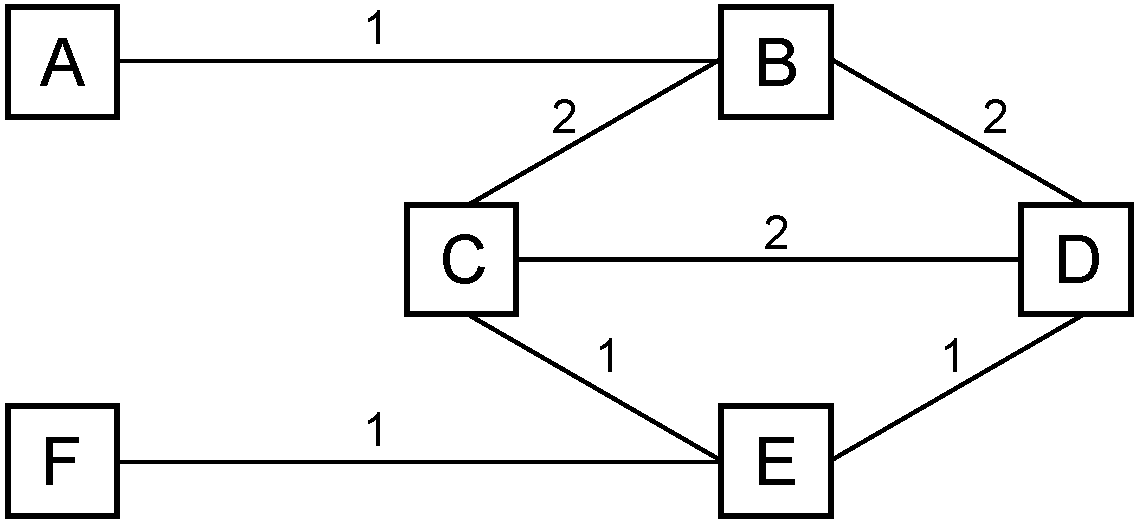
\includegraphics[width=5.5cm]{./images/zadanie02.pdf}
			\end{wrapfigure} 
			W sieci z metryką jak na rysunku routery wymieniają się informacjami co 40 sekund, stosowany jest protokół typu Distance Vector. W chwili $ t_0 $ router F ulega awarii. Określ, po jakim czasie informacja o niedostępności routera F dotrze do węzła A.\\\\\\\\
		\subsubsection{Odpowiedź}
			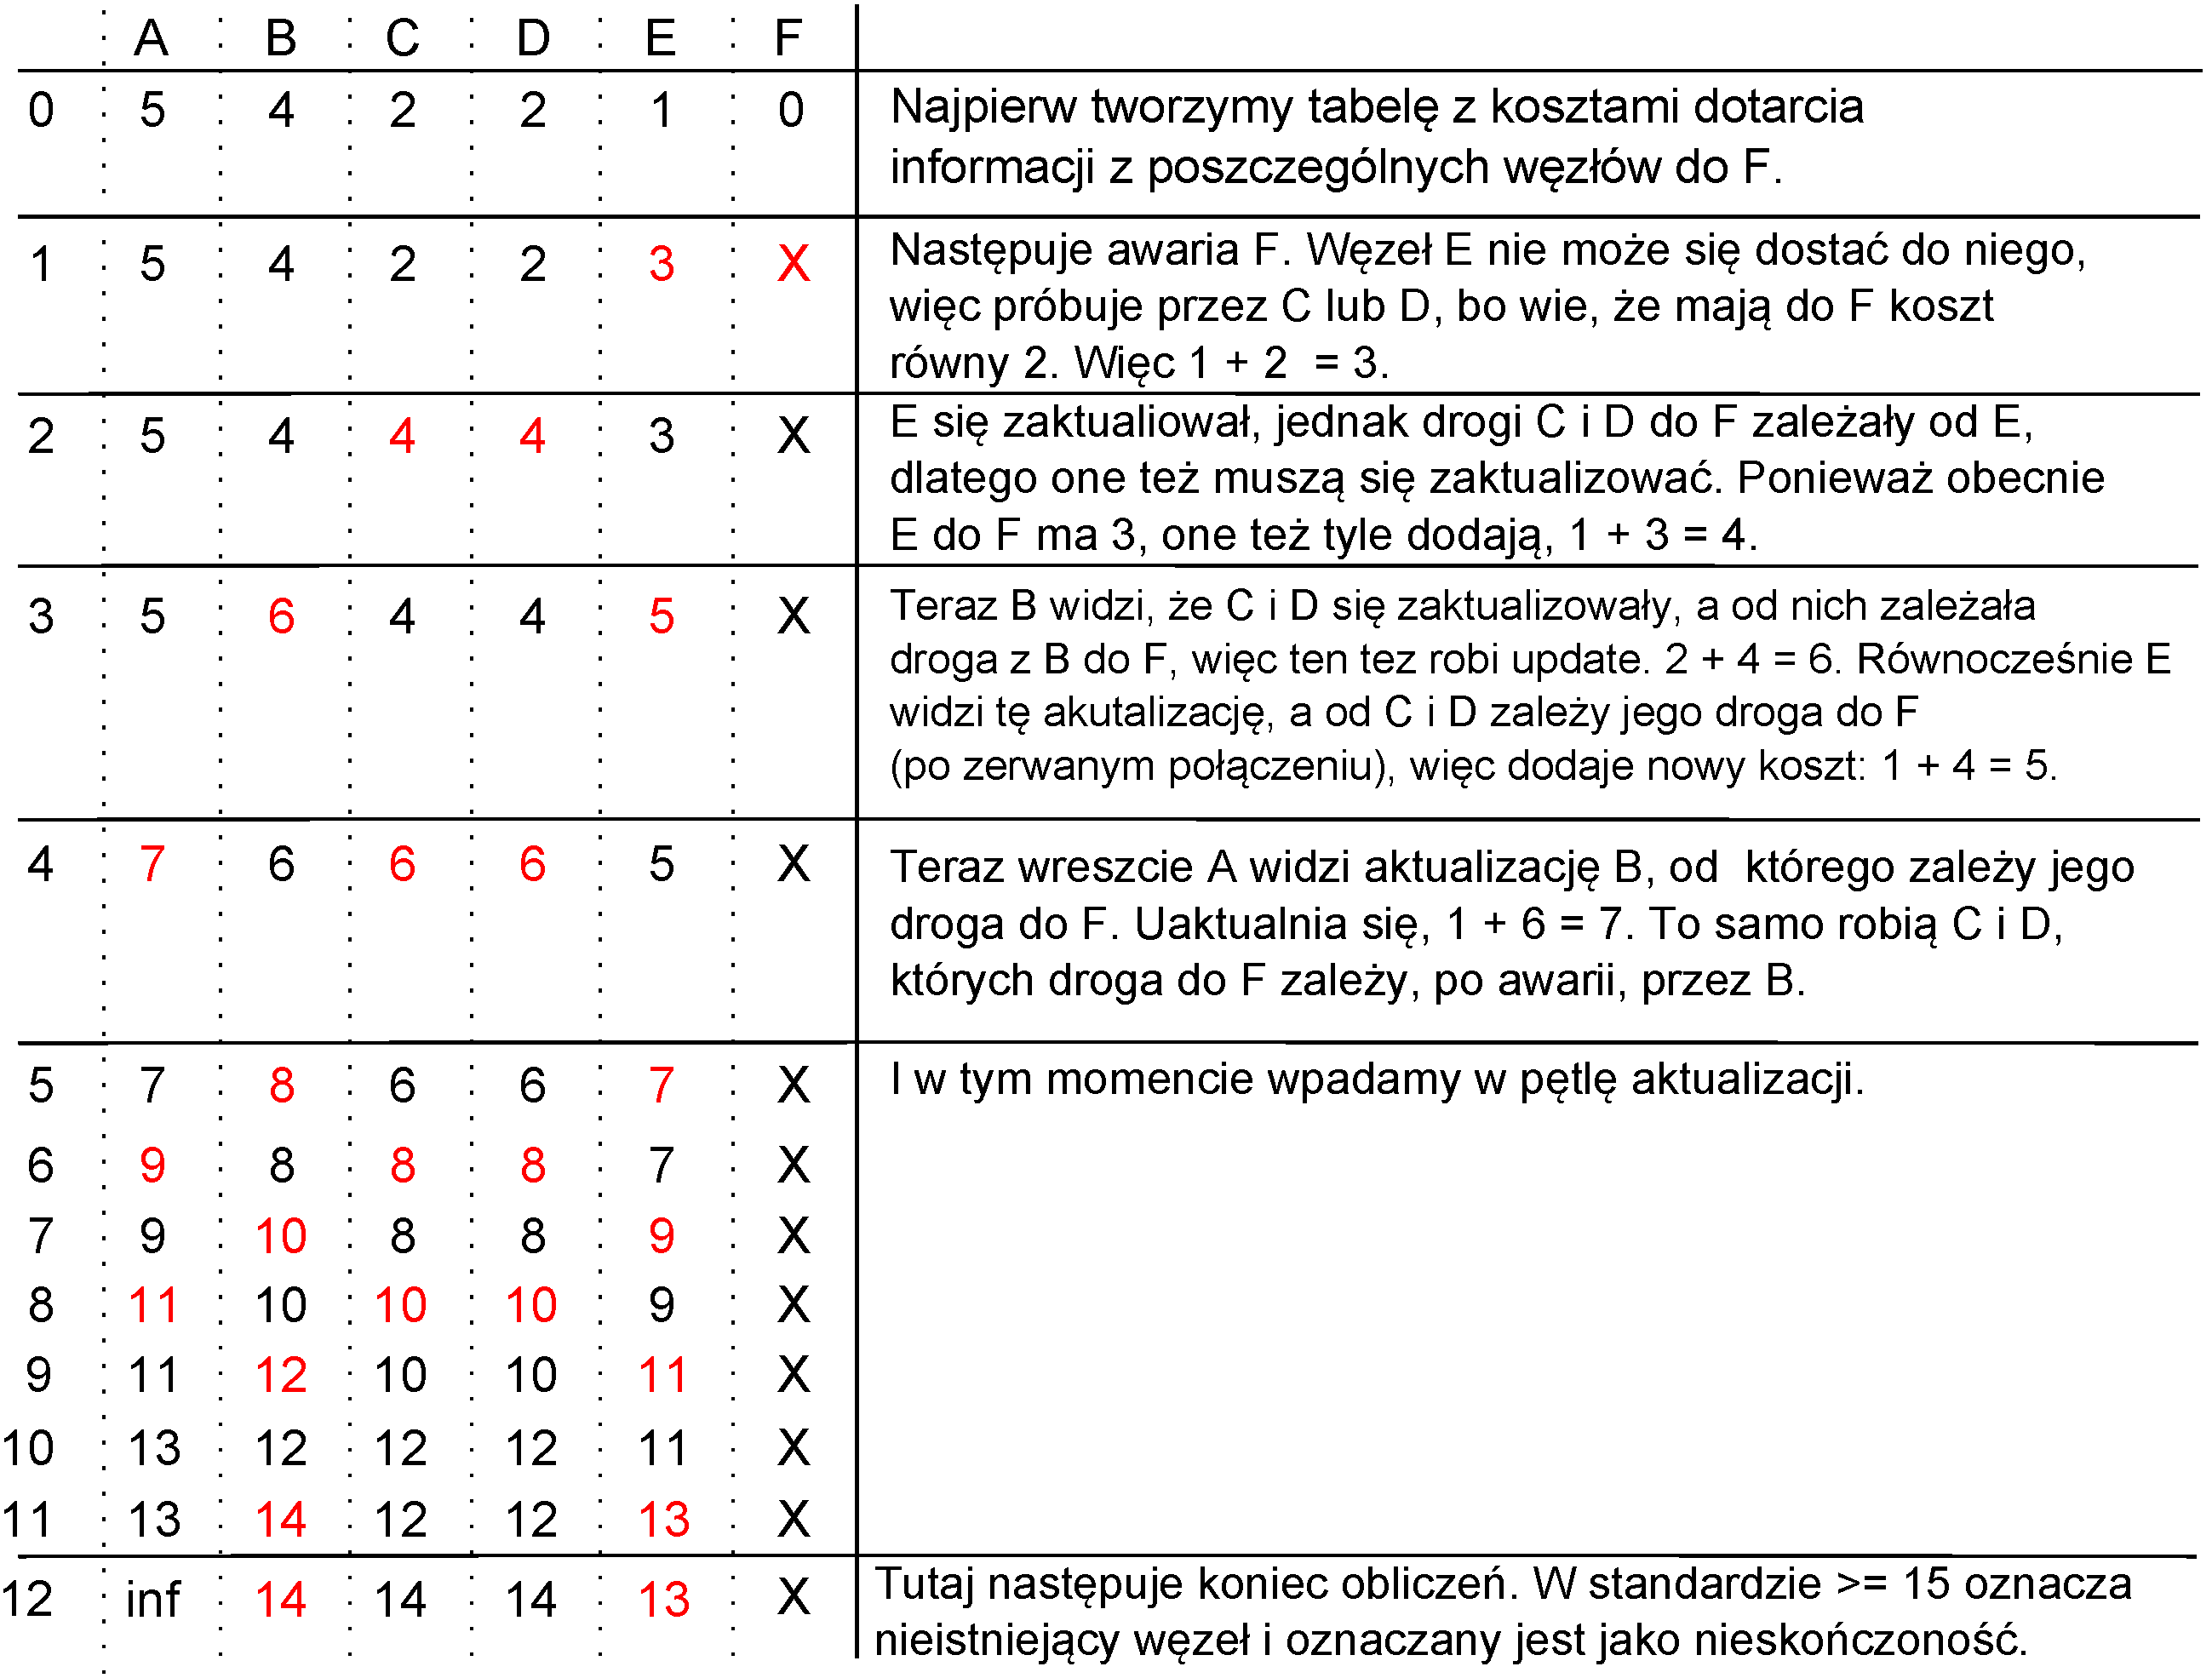
\includegraphics[width=16.0cm]{./images/zadanie03.pdf}\\
			A więc stacja A dowie się o niedostępności stacji F po $ 12\cdot 40\;s=480\;s $.
\newpage
	% ================= ZADANIE 1.2 ==================
	\subsection{Zadanie}
		\subsubsection{Treść}
			Dana jest następująca topologia sieci:
			\begin{itemize}
				\item Węzeł B ma jako sąsiadów węzły A, C i D
				\item Węzeł C ma jako sąsiadów węzły A, B, D i E
				\item Węzeł D ma jako sąsiadów węzły A, B, C i E
				\item Węzeł E ma jako sąsiadów węzły C i D
			\end{itemize}
			W chwili $ t_0 $ węzeł B ulega awarii. Przedstaw sposób rozchodzenia się tej informacji między węzłami, po jakim czasie informacja o tym dotrze do węzła E, jeśli w sieci stosowany jest protokół RIP typu Distance Vector i cykl wymiany wektorów wynosi 30 s. Przyjmij metrykę jednostkową łączy.
		\subsubsection{Odpowiedź}
			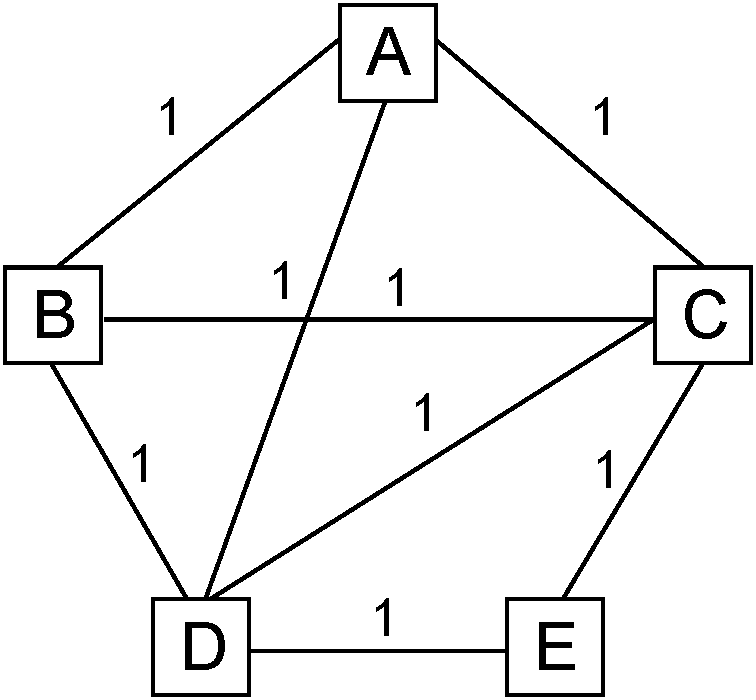
\includegraphics[width=5.0cm]{./images/zadanie04.pdf}\\\\
			\begin{tabular}{|c|c|c|c|c|c|p{7cm}|}
				\hline \textbf{Zmiana} & \textbf{A} & \textbf{B} & \textbf{C} & \textbf{D} & \textbf{E} & \textbf{Komentarz} \\ 
				\hline \textbf{0} & 1 & \color{red}{X} & 1 & 1 & 2 & Moment awarii \\ 
				\hline \textbf{1} & \color{red}{2} & X & \color{red}{2} & \color{red}{2} & 2 & B ulega awarii. Sąsiedzi, czyli A, C i D próbują połączyć się z przez swoich sąsiadów. \\ 
				\hline \textbf{2} & \color{red}{3} & X & \color{red}{3} & \color{red}{3} & \color{red}{3} & Węzły aktualizują się wzajemnie oraz E musi zrobić swoją. \\ 
				\hline \textbf{3} & \color{red}{4} & X & \color{red}{4} & \color{red}{4} & \color{red}{4} & I zaczyna się pętla. \\
				\hline \textbf{4} & \color{red}{5} & X & \color{red}{5} & \color{red}{5} & \color{red}{5} &  \\ 
				\hline \textbf{5} & \color{red}{6} & X & \color{red}{6} & \color{red}{6} & \color{red}{6} &  \\ 
				\hline \textbf{6} & \color{red}{7} & X & \color{red}{7} & \color{red}{7} & \color{red}{7} &  \\ 
				\hline \textbf{7} & \color{red}{8} & X & \color{red}{8} & \color{red}{8} & \color{red}{8} &  \\ 
				\hline \textbf{8} & \color{red}{9} & X & \color{red}{9} & \color{red}{9} & \color{red}{9} &  \\ 
				\hline \textbf{9} & \color{red}{10} & X & \color{red}{10} & \color{red}{10} & \color{red}{10} &  \\ 
				\hline \textbf{10} & \color{red}{11} & X & \color{red}{11} & \color{red}{11} & \color{red}{11} &  \\ 
				\hline \textbf{11} & \color{red}{12} & X & \color{red}{12} & \color{red}{12} & \color{red}{12} &  \\ 
				\hline \textbf{12} & \color{red}{13} & X & \color{red}{13} & \color{red}{13} & \color{red}{13} &  \\ 
				\hline \textbf{13} & \color{red}{14} & X & \color{red}{14} & \color{red}{14} & \color{red}{14} &  \\ 
				\hline \textbf{14} & \color{red}{15} & X & \color{red}{15} & \color{red}{15} & \color{red}{15} &  Koniec. \\
				\hline 
			\end{tabular}\\\\
			Obliczenia kończą się, gdy koszt trasy z węzła E do B przekroczy 15. Wówczas widzimy, że dokonanych zmian było 14, a więc czas wynosi: $ 14\cdot 30\;s=420\;s=7$ minut.

% ==================================================
% --- 2. ETHERNET
% ==================================================
\section{Ethernet}
	% ================= ZADANIE 2.1 ==================
	\subsection{Zadanie}
		\subsubsection{Treść}
			Kontroler karty sterownika sieci Ethernet odebrał następujące ramki:
			\begin{enumerate}
				\item Długość 51 bajtów, poprawne CRC
				\item Długość 39 bajtów, błędne CRC
				\item Długość 66 bajtów, poprawne CRC
				\item Długość 1510 bajtów, poprawne CRC
				\item Długość 1525 bajtów, poprawne CRC
				\item Długość 1540 bajtów, błędne CRC
			\end{enumerate}
			Jak zaklasyfikować powyższe ramki? (błąd protokołu, błąd transmisji, kolizja, poprawna ramka)
		\subsubsection{Odpowiedź}
			\begin{itemize}
				\item Jeśli ramka ma mniej niż 64 bajty i błędne CRC to jest to kolizja
				\item Jeśli ramka ma mniej niż 64 bajty i poprawne CRC to jest to błąd protokołu
				\item Jeśli ramka ma więcej niż 1518 bajtów, to zawsze jest to błąd protokołu, niezależnie od poprawności CRC
				\item Jeśli ramka ma niemniej 64 bajty i nie więcej niż 1518 bajtów oraz niepoprawne CRC to jest to błąd transmisji
				\item Poprawna ramka powinien mieć 64 - 1518 bajtów i poprawne CRC
			\end{itemize}
			\begin{enumerate}
				\item Błąd protokołu
				\item Kolizja
				\item Poprawna
				\item Poprawna
				\item Błąd protokołu
				\item Błąd protokołu
			\end{enumerate}
	% ================= ZADANIE 2.2 ==================
	\subsection{Zadanie}
		\subsubsection{Treść}
			W przypadku wystąpienia kolizji w segmencie sieci Ethernet czas oczekiwania na retransmisję $ T_R $ generowany jest jako liczba losowa z przedziału:
			\begin{enumerate}
				\item O stałej wielkości ustalanej przy konfiguracji sieci (jakiej?)
				\item O wielkości rosnącej liniowo z numerem kolizji
				\item O wielkości rosnącej z kwadratem numeru kolizji
				\item O wielkości rosnącej z kwadratem do pewnego numeru kolizji
			\end{enumerate}
			Jak obliczany jest czas $ T_R $?
		\subsubsection{Odpowiedź}
			Chodzi tutaj o algorytm CSMA, wykorzystywany do rozwiązywania kolizji na łączu kablowym. Wzór, o który prosi pytanie, zawarty jest w algorytmie dostępu w transmisji częściowo kontrolowanej. W pełni kontrolowanym dostępie występuje Token oraz rywalizacja stacji o dostęp (chyba o to chodzi).
			$$ T_{R} = r(x)\times (2^{k}-1)\times T_{ob}$$Gdzie:
			\begin{itemize}
				\item $ r(x) $ - liczba losowa z zakresu 0...1
				\item $ T_{ob} $ - czas obiegu łącza, w najgorszym wypadku podwojony czas propagacji
				\item $ k $ - liczba kolizji, czyli który raz się te ramki już zderzyły.
				\item Wraz ze zwiększaniem się liczby kolizji, możliwy zakres rośnie ekspotencjalnie. Jednak maksymalna wielkość $ k $ jest równa \textbf{10}. Dla $ k > 10 $ przyjmuje się $ k=10 $.
				\item Próbujemy szczęścia aż $ k < 15 $, potem próby są przerywane.
			\end{itemize}
			Dlatego poprawna odpowiedź to: \textit{Czas oczekiwania na retransmisję $ T_R $ generowany jest jako liczba losowa z przedziału \textbf{o wielkości rosnącej z kwadratem do pewnego numeru kolizji, \underline{a tym numerem jest 10}}}\\
			{\small \emph{Forczu: jeszcze to sprawdzę}}.
	% ================= ZADANIE 2.3 ==================
	\subsection{Zadanie}
		\subsubsection{Treść}
			Chcemy zastosować protokół CSMA / CD przy budowie sieci o długości łącza 500 m przy szybkości transmisji 200 MBit/s. Jaka powinna być w tym przypadku minimalna długość ramki?
		\subsubsection{Odpowiedź}
		\begin{enumerate}
			\item \textbf{Pierwsza metoda:}\\
			Najpierw liczymy czas propagacji $$ t_p = \cfrac{dystans}{predkosc\_lacza} $$
			Prędkości łącza nie mylić z szybkością transmisji. W przypadku światłowodu wynosi ono 2/3 prędkości światła czyli 200 000 000 m/s, tu takie założenie można dać. O tej wartości należy pamiętać na sztywno. Następnie liczmy czas propagacji sygnału przez 500 [m]:
			$$ t_p=\frac{500\;[m]}{200\:000\:000\:[m/s]}=2.5\:\mu s $$
			W obie strony czas ten wynosi $ 2.5\:\mu s = 5\:\mu s$.\\
			Bierzemy czas 2 razy, ponieważ "istnieje możliwość, że dwa lub więcej urządzeń przystąpi do wysyłania danych w tej samej chwili lub zanim sygnał z pierwszego węzła dotrze do drugiego. W takiej sytuacji żadne z nich nie wykryje sygnału nośnego drugiego. W efekcie obydwa urządzenia wysyłając dane w (prawie) tym samym czasie spowodują kolizję w sieci Ethernet."\\
			Aby CSMA/CD działało poprawnie cała ramka musi być wysłana w tych $5\:\mu s$, czyli wyliczamy jej długość:
			$$ N=szybkosc\_transmisji\cdot t_p $$
			$$ N=\cfrac{5\;[\mu s]}{200\:000\:000\:[\cfrac{b}{s}]} =200\cdot5\;bit=1000\:bit=125\:B $$
			\item \textbf{Druga metoda:}\\
			\begin{itemize}
				\item $ L=500\;[m] $
				\item $ V=200\;[Mbit/s] $
				\item $ t=\cfrac{200\:000\:000\;[{m}]}{200\:000\:000\;[\cfrac{m}{s}]}=\;[s] $
				\item $ N=2\cdot500=1000 $
				\item $ \cfrac{1000}{8}=125 $ - długość ramki
			\end{itemize}
			{\small \emph{Forczu: ocenione na 1.0 / 1.0}}
		\end{enumerate}
			
	% ================= ZADANIE 2.4 ==================
	\subsection{Zadanie}
		\subsubsection{Treść}
			Określić maksymalną długość ramki powstającej w wyniku kolizji w sieci pierścieniowej o sumarycznej długości łączy $ L=6\:km $, $ n=50 $ stacji i szybkości transmisji równej 25 Mbitów/s, przy zastosowaniu rywalizacyjnego (CSMA / CD) algorytmu dostępu do łącza.
		\subsubsection{Odpowiedź}
		\begin{enumerate}
			\item Czas propagacji: $ \cfrac{\cfrac{1}{2}\cdot L}{\cfrac{2}{3}\cdot C} = \cfrac{3\:[km]}{200\:000\:000\;[\cfrac{m}{s}]}=15 [\mu s]$
			\item Liczba bitów w pierścieniu $ N_{ring} $: $ \cfrac{L}{\cfrac{2}{3}\cdot C}\cdot \cfrac{1}{V} = 30 [\mu s] \cdot \cfrac{1}{25\;[Mbit/s]}=75\;[Mbit] $
			\item Rozmiar ramki: $ 25\;[Mbit/s]\cdot 2 \cdot 15 [\mu s]=750\;[b] $
		\end{enumerate}

% ==================================================
% --- 3. TCP / IP
% ==================================================
\section{TCP / IP}
% ================= ZADANIE 3.1 ==================
\subsection{Zadanie}
	\subsubsection{Treść}
		Przedstaw i porównaj dostępne mechanizmy działania protokołu sterowania przypływem w połączeniach warstwy transportowej i w połączeniach warstwy liniowej (np. SDLC, TCP). W jaki sposób odbierająca stacja transportowa może uzyskać czasowe powstrzymanie transmisji przez nadawcę?
	\subsubsection{Odpowiedź}
		\begin{itemize}
			\item \textbf{TCP} - kontrolowanie poprzez zmianę rozmiaru okna odbiorcy.
			\item \textbf{SDLC / HDLC} - kontrolowanie przez sygnały typu WACK / ACK w protokole znakowym BSC (RR, RNR).
		\end{itemize}
		


% ==================================================
% --- 4. ROUTING
% ==================================================
\section{Routing}
	% ================= ZADANIE 4.1 ==================
	\subsection{Zadanie}
		\subsubsection{Treść}
			Opisz zasadę działa algorytmu dystrybucji pakietów Link State. Przedstaw działanie algorytmu w węźle A w przypadku, gdy węzeł ma jako sąsiadów węzły B, C, D, E i F oraz otrzymał w czasie ostatnich 5 ms pakiety z węzłów C, F i D. Przyjąć, że maksymalny czas oczekiwania na kolejne kopie to 10 ms i węzeł nie odebrał w tym czasie innych pakietów.
		\subsubsection{Odpowiedź}
				\begin{tabular}{|c|c|c|c|c|c|c|c|}
					\hline \multicolumn{2}{|c|}{\textbf{C}}  & & \multicolumn{2}{|c|}{\textbf{F}} & & \multicolumn{2}{|c|}{\textbf{D}}\\ 
					\hline \multicolumn{2}{|c|}{213} & &\multicolumn{2}{|c|}{214} & &\multicolumn{2}{|c|}{214} \\ 
					\hline \multicolumn{2}{|c|}{178} & &\multicolumn{2}{|c|}{260} & &\multicolumn{2}{|c|}{259}   \\ 
					\hline U & 3 & & U & 2 & & U & 2\\ 
					\hline V & 5 & & V & 4 & & V & 4\\
					\hline Z & 4 & & Z & 5 & & Z & 5\\
					\hline 
				\end{tabular}\\\\\\
			Przykładowy zestaw pakietów zadziała następująco: stacja A wyśle potwierdzenia do węzłów F i D. Do węzłów B, C i E wyśle pakiet z F. Dlaczego?\\
			Potwierdzenia wysyłane są do węzłów z których przyszły pakiety z najwyższym numerem sekwencyjnym (drugi wiersz). W tym przypadku są to węzły F i D, których $ seq $ są równie 214. Do sąsiadów, którzy nie otrzymali potwierdzenia (B, C i E) wysyłany jest ten spośród pakietów z najwyższym numerem sekwencyjnym, którego pole Age (trzeci wiersz) jest największe. Dlatego co tych trzech węzłów zostanie wysłany pakiet z F.\\\\
			Inna odpowiedź:\\
			"Pakiet pochodzący z węzła H zostanie odrzucony ponieważ jego numer sekwencyjny jest niższy niż numer pochodzący z F i D czyli zawiera stare dane. Do węzła F oraz D zostanie wysłane potwierdzenie, natomiast do węzłów C, E, H zostanie wysłany pakiet pochodzący z węzła F ponieważ posiada on dłuższy czas życia od pakietu z węzła D. Ten pakiet zostanie również uwzględniony w liczeniu nowej tablicy routingu w węźle A"
			{\small \emph{Forczu: ocenione na 1.0 / 1.0}}
\newpage
	% ================= ZADANIE 4.2 ==================
	\subsection{Zadanie}
		\subsubsection{Treść}
			Węzeł W ma za sąsiadów węzły A, B, C, D i E. Po otrzymaniu pakietu Link State węzeł oczekuje 35 ms, następnie przystępuje do dystrybucji pakietu. W chwili $ t_0 $ węzeł odebrał pakiet z węzła B, $ 5\;ms $ później z węzła D, a po 13 $ ms $ pakiet z węzła E. Przedstaw przebieg dystrybucji pakietów\\.
			\begin{tabular}{|c|c|c|c|c|c|c|c|}
				\hline \multicolumn{2}{|c|}{\textbf{E}}  & & \multicolumn{2}{|c|}{\textbf{B}} & & \multicolumn{2}{|c|}{\textbf{D}}\\ 
				\hline \multicolumn{2}{|c|}{55} & &\multicolumn{2}{|c|}{55} & &\multicolumn{2}{|c|}{55} \\ 
				\hline \multicolumn{2}{|c|}{240} & &\multicolumn{2}{|c|}{238} & &\multicolumn{2}{|c|}{239}   \\ 
				\hline U & 2 & & U & 1 & & U & 2\\ 
				\hline V & 3 & & V & 2 & & V & 3\\
				\hline Z & 6 & & Z & 5 & & Z & 6\\
				\hline 
			\end{tabular}
		\subsubsection{Odpowiedź}
			Do węzłów, których pakiety miały największy nr sekwencyjny (2gi wiersz) wysyła potwierdzenie
			Do pozostałych wysyła pakiet tego węzła, który miał największy nr sekwencyjny i age (3ci wiersz).
			\begin{itemize}
				\item Do węzła D wyśle: potwierdzenie.
				\item Do węzła C wyśle: E.
				\item Do węzła B wyśle: potwierdzenie.
				\item Do węzła E wyśle: potwierdzenie.
				\item Do węzła A wyśle: E.
			\end{itemize}
	% ================= ZADANIE 4.3 ==================
	\subsection{Zadanie}
		\subsubsection{Treść}
			\begin{wraptable}{r}{5.5cm}
				\begin{tabular}{|c|c|}
					\hline \multicolumn{2}{|c|}{Q}  \\ 
					\hline \multicolumn{2}{|c|}{1}  \\ 
					\hline \multicolumn{2}{|c|}{300}  \\ 
					\hline T & 2 \\ 
					\hline U & 1 \\ 
					\hline Z & 3 \\ 
					\hline 
				\end{tabular}
			\end{wraptable}
			Węzeł Q generuje co 60 sekund pakiety Link State, w chwili $ t_0 $ rozesłał pakiet
			$$ (Q\;|\;seq=23321\;|\;age=300\;|\;(U|3)\;|\;(V|2)\;|\;(Z|5)\;) $$
			Po restarcie w chwili $ t_0+25\;s $ wysłał pakiet
			$$ (Q\;|\;seq=1\;|\;age=300\;|\;(T|2)\;|\;(U|1)\;|\;(Z|3)\;) $$
			a potem kolejne. Przedstaw przebieg dystrybucji tej informacji w sieci. Kiedy te zmiany w topologii zostaną uwzględnione w wyznaczaniu tablicy routingu?
		\subsubsection{Odpowiedź}
			Działanie Link State:
			\begin{itemize}
				\item "Powiedz wszystkim o swoich sąsiadach" - przekazuje pakiety otrzymane od sąsiednich węzłów do sąsiednich węzłów.
				\item Nr sekwencyjny - jeśli ktoś dostanie pakiet o większym numerze, to go przetwarza (i przesyła dalej), a jeśli nie jest większy, to nie.
				\item Wiek - czas życia pakietu (w cyklu). Jeśli czas życia upływa to jest usuwany z tablicy routingu. Liczony w sekundach.
			\end{itemize}
\newpage
			\textbf{Odpowiedzi}:
			\begin{enumerate}
				\item Węzły odrzucają pakiet z niższym numerem sekwencyjnym, więc nowy pakiet będzie uwzględniony po wygaśnięciu wa(żności?) pierwszego, czyli za $ 275\;s $.\\
				\small{ \emph{Ocenione na 0.9 / 1.0}}
				\item \small{ \emph{Forczu:}} dlaczego ujebano ten 0.1? Wg mnie dlatego, że kruczek tkwi w słowie "reset". Pakiety są wysyłane co 60 sekund, ale od momentu resetu ($ t_0+25\;s $) zaczynamy liczyć od nowa, czyli nowe pakiety są wysyłane w momentach $ 85\;s, 145\;s, 205\;s $ itd.\\
				Dlatego prawidłową odpowiedzią imo jest $ t_0+25+\textbf{5}\cdot{60}=325\;s $, czyli dopiero \textbf{5ty} pakiet zostanie uwzględniony przez tablicę routingu.
				\item \small{ \emph{Inna odpowiedź, ocena nienzna:}}\\
				W momencie restartu, po 25 sekundach, oba pakiety żyją i ważniejszy jest Pierwszy z nich, o numerze sekwencyjnym $ seq=23321 $. Dlatego pakiet o $ seq=1 $ zostanie uwzględniony po przedawnieniu $ seq=23321 $, czyli po:
				$$ 300 - 25 - t_0\;[s]= 275\;[s] $$
				a najpierw zostanie wykorzystany pakiet o $ seq=23321 $.
				\item \emph{by Forczu}: tablica po uwzględnieniu pakiet o $ seq=23321 $ \\
					\begin{tabular}{|c|c|}
						\hline \multicolumn{2}{|c|}{Q}  \\ 
						\hline \multicolumn{2}{|c|}{1}  \\ 
						\hline \multicolumn{2}{|c|}{300}  \\ 
						\hline U & 1 \\
						\hline V & 2 \\
						\hline Z & 3 \\ 
						\hline 
					\end{tabular}\\\\
				Nowe $ U=3 $, czyli koszt jest wyższy od obecnego, więc nie jest uwzględnione.\\
				Nowe $ Z=5 $, czyli to samo co wyżej.\\
				Nowe $ V=5 $, tego nie ma w obecnej tablicy, więc po prostu jest dodane.
		\end{enumerate}
	% ================= ZADANIE 4.4 ==================
	\subsection{Zadanie}
		\subsubsection{Treść}
			Węzeł D odebrał / wysłał do chwili $ T_0 $ następujące pakiety.\\
			\begin{tabular}{|c|c|c|c|c|c|c|c|c|c|c|c|c|c|c|c|c|c|c|c|c|c|c|c|c|c|c|c|c|}
				\cline{1-2} \cline{4-5} \cline{7-8} \cline{10-11} \cline{13-14} \cline{16-17} \cline{19-20} \cline{22-23} \cline{25-26} \cline{28-29}
				\multicolumn{2}{|c|}{G} &  & \multicolumn{2}{c|}{B}  &  & \multicolumn{2}{c|}{C} &  & \multicolumn{2}{c|}{E}  &  & \multicolumn{2}{c|}{D}  &  & \multicolumn{2}{c|}{F}  &  & \multicolumn{2}{c|}{A}  &  & \multicolumn{2}{c|}{H}  &  & \multicolumn{2}{c|}{C}  &  & \multicolumn{2}{c|}{B} \\ \cline{1-2} \cline{4-5} \cline{7-8} \cline{10-11} \cline{13-14} \cline{16-17} \cline{19-20} \cline{22-23} \cline{25-26} \cline{28-29} 
				\multicolumn{2}{|c|}{9} &  & \multicolumn{2}{c|}{8}  &  & \multicolumn{2}{c|}{9} &  & \multicolumn{2}{c|}{8}  &  & \multicolumn{2}{c|}{9}  &  & \multicolumn{2}{c|}{14} &  & \multicolumn{2}{c|}{10} &  & \multicolumn{2}{c|}{9}  &  & \multicolumn{2}{c|}{10} &  & \multicolumn{2}{c|}{7} \\ \cline{1-2} \cline{4-5} \cline{7-8} \cline{10-11} \cline{13-14} \cline{16-17} \cline{19-20} \cline{22-23} \cline{25-26} \cline{28-29} 
				\multicolumn{2}{|c|}{3} &  & \multicolumn{2}{c|}{25} &  & \multicolumn{2}{c|}{7} &  & \multicolumn{2}{c|}{28} &  & \multicolumn{2}{c|}{29} &  & \multicolumn{2}{c|}{21} &  & \multicolumn{2}{c|}{23} &  & \multicolumn{2}{c|}{24} &  & \multicolumn{2}{c|}{23} &  & \multicolumn{2}{c|}{6} \\ \cline{1-2} \cline{4-5} \cline{7-8} \cline{10-11} \cline{13-14} \cline{16-17} \cline{19-20} \cline{22-23} \cline{25-26} \cline{28-29} 
				F          & 1          &  & A           & 3         &  & B          & 1         &  & A           & 1         &  & C           & 2         &  & A           & 1         &  & E           & 1         &  & B           & 1         &  & B           & 3         &  & A          & 1         \\ \cline{1-2} \cline{4-5} \cline{7-8} \cline{10-11} \cline{13-14} \cline{16-17} \cline{19-20} \cline{22-23} \cline{25-26} \cline{28-29} 
				H          & 1          &  & H           & 2         &  & E          & 2         &  & C           & 2         &  & H           & 1         &  & E           & 1         &  & B           & 2         &  & G           & 2         &  & E           & 1         &  & H          & 1         \\ \cline{1-2} \cline{4-5} \cline{7-8} \cline{10-11} \cline{13-14} \cline{16-17} \cline{19-20} \cline{22-23} \cline{25-26} \cline{28-29} 
				D          & 1          &  & C           & 2         &  & D          & 2         &  & F           & 1         &  & G           & 1         &  & G           & 1         &  & F           & 2         &  & D           & 2         &  & D           & 1         &  & C          & 2         \\ \cline{1-2} \cline{4-5} \cline{7-8} \cline{10-11} \cline{13-14} \cline{16-17} \cline{19-20} \cline{22-23} \cline{25-26} \cline{28-29}
				\multicolumn{2}{c}{1} &  & \multicolumn{2}{c}{2} &  & \multicolumn{2}{c}{3} &  & \multicolumn{2}{c}{4} &  & \multicolumn{2}{c}{5} &  & \multicolumn{2}{c}{6} &  & \multicolumn{2}{c}{7} &  & \multicolumn{2}{c}{8} &  & \multicolumn{2}{c}{9} &  & \multicolumn{2}{c}{10} \\ 
			\end{tabular}\\
			W czasie $ T_0+5 $ węzeł D rozpoczął wyznaczanie nowej tablicy routingu. Przedstawić nową tablicę routingu dla węzła D.
\newpage
		\subsubsection{Odpowiedź}
			Format pakiety wyraźnie wskazuje, że mamy do czynienia z algorytmem Link State.
			\begin{itemize}
				\item Pierwsza wartość oznacza nadawcę.
				\item Druga wartość to numer sekwencyjny - im większy tym pakiet jest ważniejszy.
				\item Trzecia wartość to wiek - po tego upływie czasu od momentu odebrania pakiet jest usuwany.
			\end{itemize}
			A więc przed rozpoczęciem wyznaczania topologii sieci:
			\begin{enumerate}
				\item Na samym początku \textbf{odrzucamy} pakiety nr 1 o czasie życia 3 - w momencie wyznaczania nowej tablicy, w momencie $ T_0+5 $ już nie istniał.
				\item Następnie patrzymy na numery sekwencyjne - jeżeli odebraliśmy 2+ pakietów od tego samego węzła, to interesuje nas tylko ten o najwyższym numerze sekwencyjnym.
				\begin{itemize}
					\item Są dwa pakiety od węzła B, nr 2 i 10. Odrzucamy nr 10 o niższym \textit{seq} ($ 8 > 7 $).
					\item Są dwa pakiety od węzła C, nr 3 i 9. Odrzucamy nr 3 o niższym \textit{seq} ($ 9 < 10 $).
				\end{itemize}
				\item Odrzucamy te węzły, do których istnieje droga z pakietów innych węzłów, ale owe węzły już nie istnieją, bo zostały odrzucone w dwóch poprzednich krokach. W topologii skutkuje to tylko pojedynczą drogą z jednego węzła do drugiego, a interesują nas tylko te z dwiema możliwościami.
			\end{enumerate}
			Do obliczeń przystępujemy z 7 pakietami. Wszystko sobie rozrysowujemy:\\
				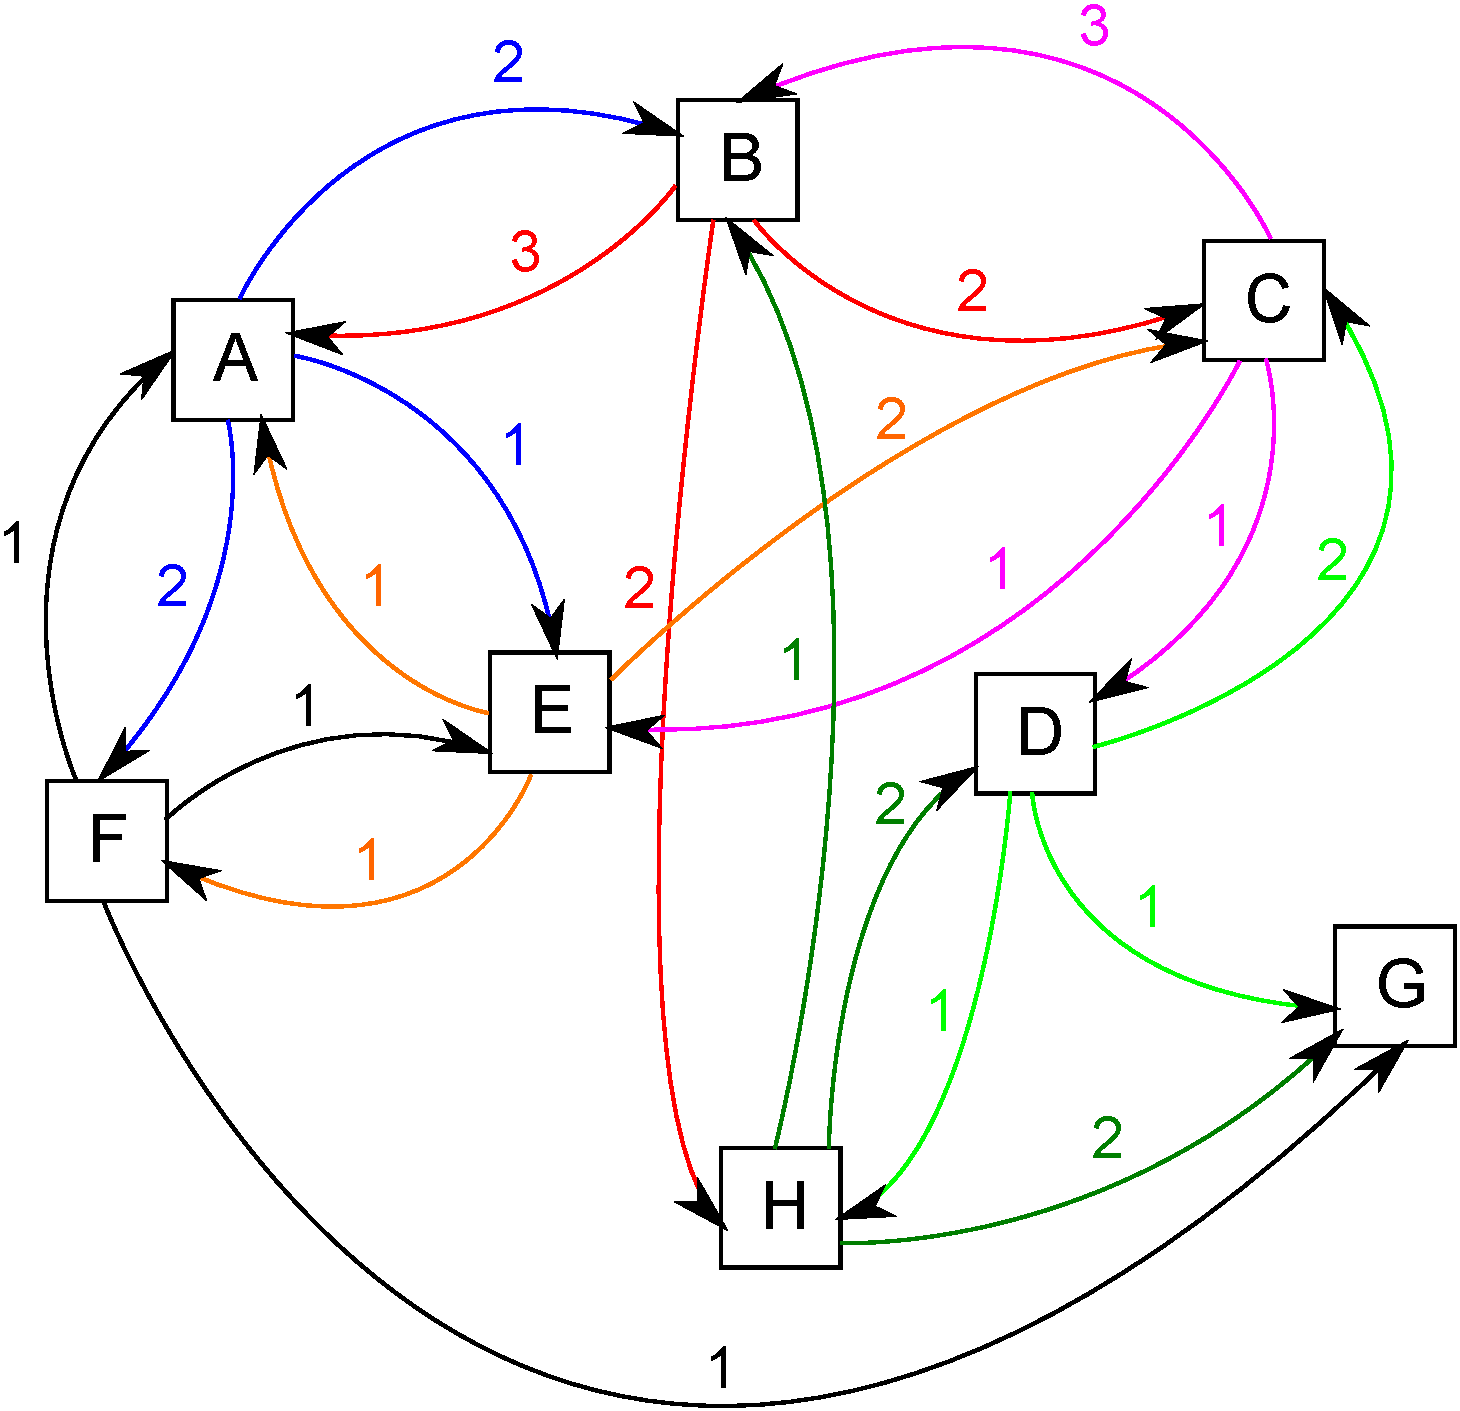
\includegraphics[width=8.0cm]{./images/zadanie05.pdf}
				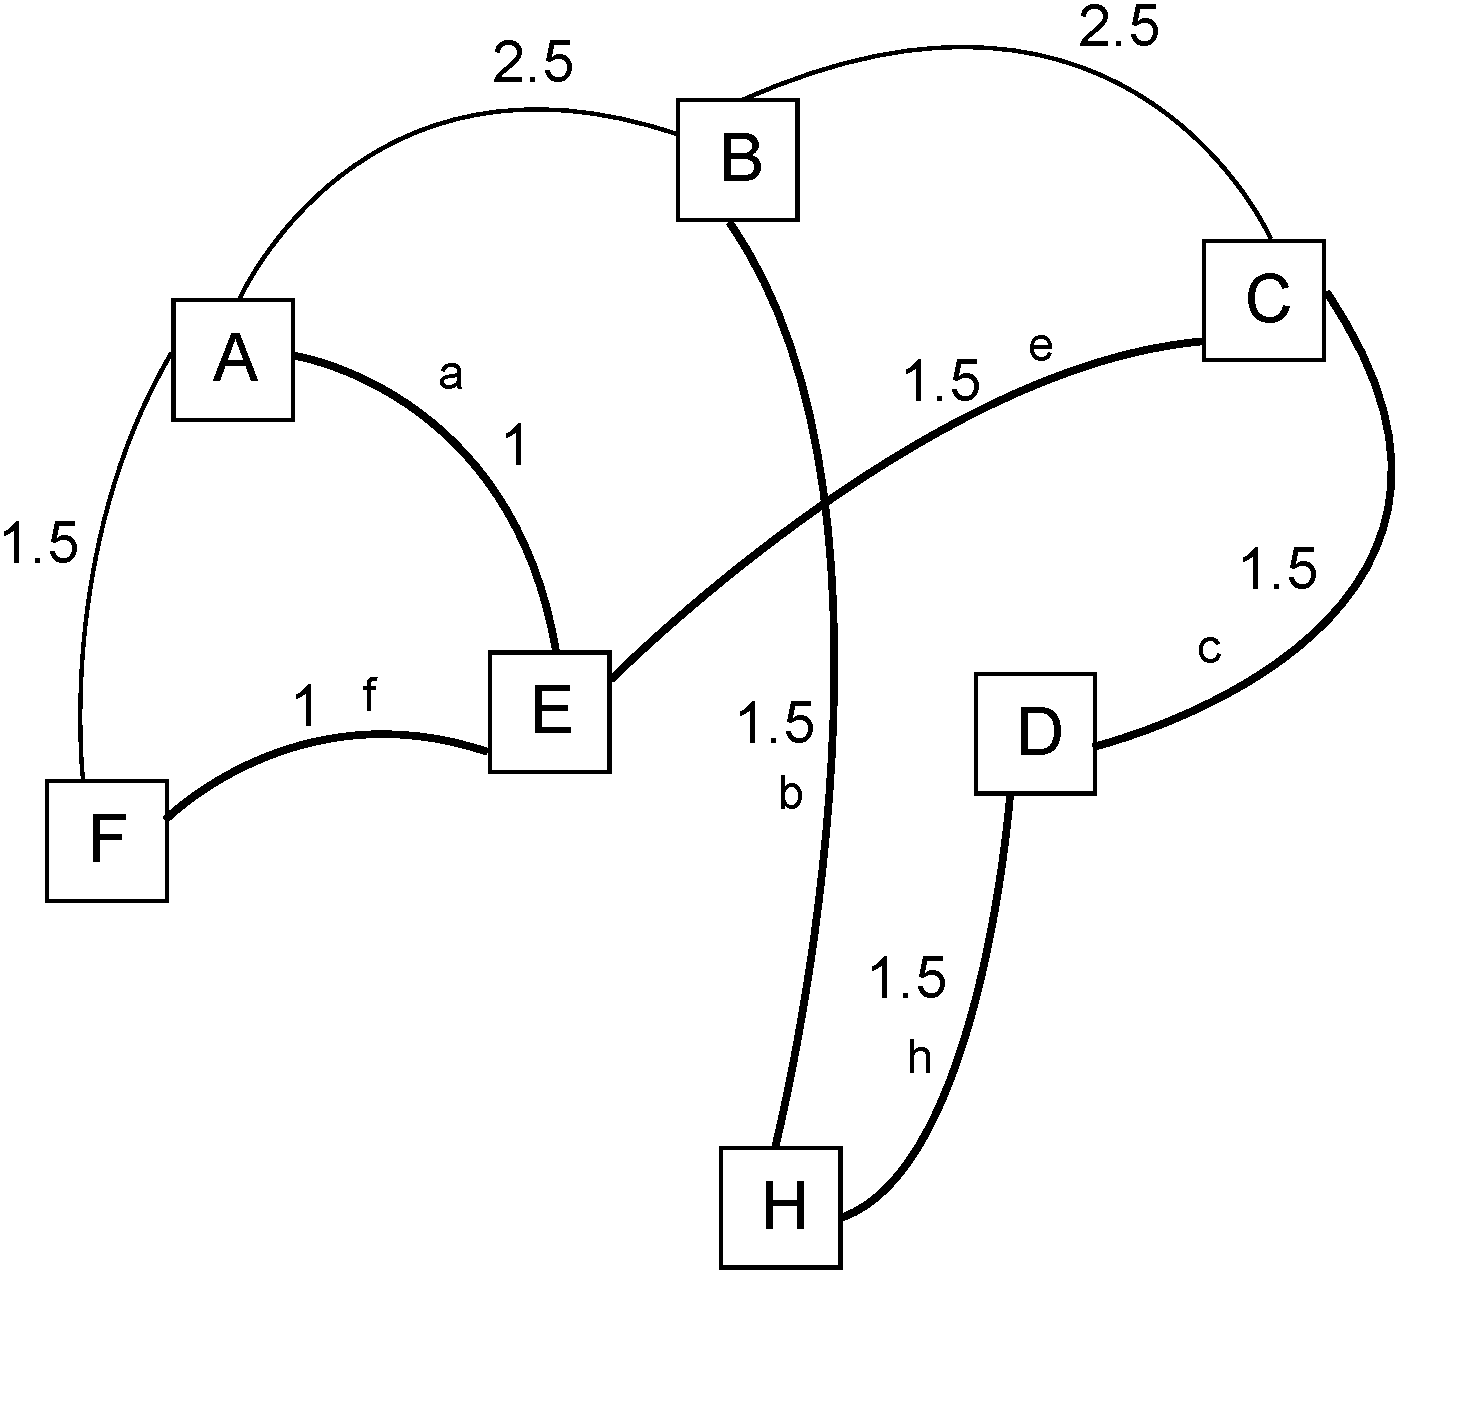
\includegraphics[width=8.0cm]{./images/zadanie06.pdf}\\
			Jeśli węzły da się połączyć na dwa różne sposoby, tworzymy średnią arytmetyczną. Wybieramy najkrótsze możliwe połączenie do każdego węzła, \textbf{pomijamy G}, i rysujemy tabelkę.\\\\ 
			\begin{tabular}{c|c|c}
				Cel & Koszt & Przez \\ \hline
				A   & 4     & E     \\
				B   & 3     & H     \\
				C   & 1.5   & D     \\
				D   & 0     &       \\
				E   & 3     & C     \\
				F   & 4     & E     \\
				G   & -     &       \\
				H   & 1.5   & D     
			\end{tabular}\\
			\small{ \emph{Forczu: ocenione na 1.0 / 1.0\\
					Podobno uwzględnienie G to 0.0 / 1.0}}.
	% ================= ZADANIE 4.5 ==================
	\subsection{Zadanie}
		\subsubsection{Treść}
			Węzeł K po restarcie wysłał do sąsiadów L, I, F swoją początkową tablicę routingu i otrzymał od nich ich tablice routingu. Wyznacz nową tablicę routingu węzła K.\\\\
			\begin{tabular}{cc m{1cm}|c|c|c|c|c|ccc}
				\cline{1-2} \cline{4-5} \cline{7-8} \cline{10-11}
				\multicolumn{2}{|c|}{\textbf{K}}                 &  & \multicolumn{2}{c|}{\textbf{L}} &  & \multicolumn{2}{c|}{\textbf{F}} & \multicolumn{1}{c|}{} & \multicolumn{2}{c|}{\textbf{I}}                 \\ \cline{1-2} \cline{4-5} \cline{7-8} \cline{10-11} 
				\multicolumn{1}{|c|}{I} & \multicolumn{1}{c|}{1} &  & D              & 3              &  & A              & 3              & \multicolumn{1}{c|}{} & \multicolumn{1}{c|}{J} & \multicolumn{1}{c|}{2} \\ \cline{1-2} \cline{4-5} \cline{7-8} \cline{10-11} 
				\multicolumn{1}{|c|}{F} & \multicolumn{1}{c|}{2} &  & C              & 4              &  & B              & 2              & \multicolumn{1}{c|}{} & \multicolumn{1}{c|}{H} & \multicolumn{1}{c|}{3} \\ \cline{1-2} \cline{4-5} \cline{7-8} \cline{10-11} 
				\multicolumn{1}{|c|}{L} & \multicolumn{1}{c|}{1} &  & G              & 2              &  & C              & 1              & \multicolumn{1}{c|}{} & \multicolumn{1}{c|}{N} & \multicolumn{1}{c|}{3} \\ \cline{1-2} \cline{4-5} \cline{7-8} \cline{10-11} 
				&                        &  & H              & 1              &  & E              & 2              & \multicolumn{1}{c|}{} & \multicolumn{1}{c|}{M} & \multicolumn{1}{c|}{4} \\ \cline{4-5} \cline{7-8} \cline{10-11} 
				&                        &  & N              & 2              &  & G              & 1              & \multicolumn{1}{c|}{} & \multicolumn{1}{c|}{E} & \multicolumn{1}{c|}{3} \\ \cline{4-5} \cline{7-8} \cline{10-11} 
				&                        &  & M              & 5              &  & J              & 2              &                       &                        &                        \\ \cline{4-5} \cline{7-8}
			\end{tabular}
		\subsubsection{Odpowiedź}
		\begin{wraptable}{l}{5.5cm}
			\begin{tabular}{c|c|c}
				Do & Przez & Koszt \\ \hline
				A  & F     & 5     \\
				B  & F     & 4     \\
				C  & F     & 3     \\
				D  & L     & 4     \\
				E  & F     & 4     \\
				F  & -     & 2     \\
				G  & L     & 3     \\
				H  & L     & 2     \\
				I  & -     & 1     \\
				J  & I     & 3     \\
				K  & -     & -     \\
				L  & -     & 1     \\
				M  & I     & 5     \\
				N  & L     & 3    
			\end{tabular}
		\end{wraptable}
		W tym wszystkim interesują nas tylko drogi lokalnie najbliższe - te z punktu widzenia węzła K i "ofert" dróg sąsiadów. Jeśli dwie drogi mają ten sam koszt to wybór powinien być obojętny. Sąsiedzi (L, I, F) mają się w końcowej tabeli również znajdować.\\
		\small{ \emph{Forczu: ocenione na 1.0 / 1.0}}.\\\\\\\\\\\\\\\\\\\\\\\\
		
\newpage
% ==================================================
% --- 5. TRANSMISJA DANYCH
% ==================================================
\section{Transmisja danych}
% ================= ZADANIE 5.1 ==================
	\subsection{Zadanie}
		\subsubsection{Treść}
			Stacja robocza jest połączona z serwerem z prędkością 11 [Mbps] i stopą błędów BER = $ 7.3 \cdot 10 ^ {-6} $. Oblicz z jaką średnią prędkością mogą być wysyłane informacje z serwera używając wersji standardowej (\emph{plain vanilla}, \emph{Go Back N}) protokołu TCP. Wynegocjowany segment danych to 768 [B] (ramka w łączu 832 [B]), rozmiar okna to 18.5 [KB], a średni czas RTT to 55 [ms].
		\subsubsection{Odpowiedź}
			\begin{enumerate}
				\item Notacja BER = $ 7.3 \cdot 10 ^ {-6} $ oznacza, że na 1 milion bitów 7.3 z nich są przekłamane. Wyliczamy z nich liczbę przekłamanych bajtów. Dzielimy obie strony przez 7.3, czyli 1 na 136986.3 bitów jest nieprawidłowy. Aby uzyskać bajty, dzielimy oba przez 8, czyli 1 na 17123.3 bajtów jest przekłamany.
				\item Wyliczamy z tego liczbę przekłamanych ramek:
				$$ \cfrac{17123.3\;[B]}{832\;[B]}\approx20.58 $$
				Wybieramy ramkę w łączu, ponieważ interesują nas przesyłane informacje. Wynik oznacza, że 1 z 21 ramek jest przekłamana.
				\item Teraz liczymy liczbę ramek jaka pomieści się w oknie:
				$$ \cfrac{18.5\;[kB]}{768\;[B]}=\cfrac{18\:944\;[B]}{768\;[B]}\approx24.67 $$
				Wybieramy liczbę danych w segmencie, ponieważ interesuje nas to co może pomieścić okno. Z obliczeń wynika, że wielkość okna jest równa 24 ramki + kawałek 25ej, połowa z tego to 12.
				\item Możemy przystąpić do rysowania słupków:
				\begin{center}
					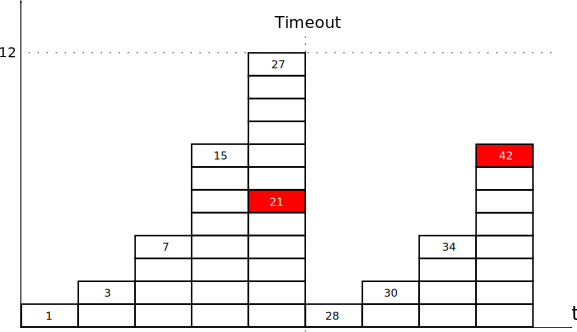
\includegraphics[width=10.0cm]{./images/zadanie16}
				\end{center}
				Liczba ramek rośnie eksponencjalne aż napotka limit w postaci \emph{slow start threshold}u. Nie przekracza go. Gdyby w piątej kolumnie nie wystąpił błąd, liczba ramek w kolejnych rosłaby liniowo. Wówczas, po napotkaniu błędu we wzroście liniowym, \emph{treshold} do kolejnego timeoutu byłby mniejszy o połowę.
				\item Można przystąpić do wyliczenia szybkości:
				$$ SRET=\cfrac{(42-2)\cdot832\;[B]}{9\cdot55\;[ms]}\approx537858.59\;[\frac{b}{s}]\approx0.5379\;[Mbps] $$
				$$ GBN=\cfrac{(42-7)\cdot832\;[B]}{9\cdot55\;[ms]}\approx470626.26\;[\frac{b}{s}]\approx0.47069\;[Mbps]   $$
			\end{enumerate}
				
			

% ================= ZADANIE 5.1 ==================
	\subsection{Zadanie}
		\subsubsection{Treść}
			Stacja robocza połączona jest z serwerem łączem szeregowym o przepustowości 8 MBit/s, z bitową stopą błędów $ BER=2\cdot 10^{-5} $. Określić z jaką średnią szybkością transmisji danych protokołem TCP w wersji standardowej (\emph{plain vanilla}) można uzyskać jeśli uzgodniona maksymalna wielkość segmentu wynosi 768 B (ramki w łączu 832 B), wielkość danych odbiorcy wynosi 27 kB, czas $ RTT=40\;ms $.
		\subsubsection{Odpowiedź}
			Algorytm wykonywania zadań z przekłamaniem:
			\begin{enumerate}
				\item Obliczamy liczbę przekłamań w jednostce czasu jako odwrotność BERu:
				$ \cfrac{1}{BER} = \cfrac{1}{2\cdot 10^{-5}}=50000 \rightarrow$ - oznacza to, że 1 na 50k bitów jest przekłamany $ \rightarrow $ co 6250 bajt jest przekłamany.
				\item Następnie obliczamy ile ramek zostaje przekłamanych jako:
				$$ \cfrac{Odwrotnosc\;BERu}{Rozmiar\;ramki\;w\;laczu} $$
				W naszym przypadku jest to $ \cfrac{6250\;[B]}{832\;[B]}=7.51$
				\item Powyższy wynik oznacza, że 7 ramek zostało wysłanych poprawie, a 8 jest przekłamana. Czyli zakładamy, że \textbf{co 8 ramka} jest błędna (bierzemy sufit wyniku).
				\item Obliczamy liczbę ramek jaką można maksymalnie przesłać w jednym RTT jako:
				$$ \cfrac{Rozmiar\;okna}{Rozmiar\;ramki\;w\;laczu} $$
				Czyli u nas: $ \cfrac{27\:000}{832}\approx32 $
				\item Następnie stosujemy \textbf{metodę słupków} do wyznaczenia właściwego stosunku liczby ramek, jakie można wysłać.
				\begin{enumerate}
					\item Rysujemy kolejne transmitowane ramki w postaci słupków złożonych z $ 2^n $ ramek: 1, 2, 4, 8 itd.
					\begin{enumerate}
						\item Jeżeli protokół jest typu \emph{slow start} - naliczamy bezwzględnie wg $ 2^n $ - kolejne słupki mają 16, 32 itd. wysokości
						\item Jeżeli protokół jest typu \emph{congestion avoidance} - po przekroczeniu połowy okna zaczynamy zwiększać wysokość \textbf{liniowo}, czyli np. dla granicy (\emph{thresholdu}) 8 kolejne słupki będą mieć 9, 10, 11 itd. wysokości.
						\item \emph{Congestion avoidance} wykorzystujemy, gdy w poleceniu mamy bufor (podobno).
					\end{enumerate}
					\item Gdy napotykamy przekłamaną ramkę zaczynamy naliczać od nowa.
					\item Liczba ramek w słupku nie może przekroczyć maksymalnej liczby ramek jaką można wysłać w czasie RTT.
					\item Kończymy naliczanie gdy przekłamana ramka znajdzie się na szczycie jednego ze słupków, czyli po zakończeniu jednego cyklu.
				\end{enumerate}
				\item Przystępując do rysowania słupków należy zaznaczyć jaki algorytm wybraliśmy. Niech będzie "slow start", ale podobno jest zalecany CA na examie.\\
				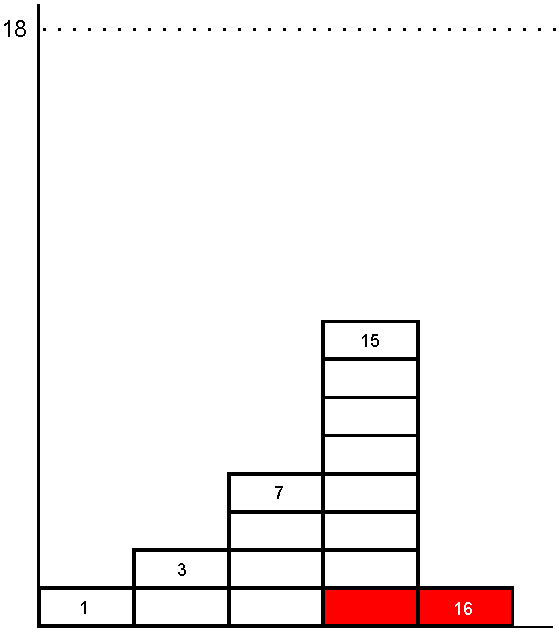
\includegraphics[width=6.0cm]{./images/zadanie07.pdf}\\\\
				Wynika z tego, że na 16 pakietów 2 zostają przekłamane. $ 16 - 2 = 14 $ - nieprzekłamane pakiety. Liczba ta nie powinna zostać przekroczona w wysyłaniu danych do okna.
				\item Na koniec pozostaje obliczyć efektywną prędkość. Może ona zostać obliczona wg dwóch wzorów:
				\begin{enumerate}
					\item \textbf{SRET}
					$$ SRET=\frac{((Liczba\;ramek - liczba\;ramek\;przekłamanych)\cdot Rozmiar\;segmentu}{Liczba\;kolumn\;w\;cyklu\cdot RTT} $$
					\item \textbf{GBN} - Go-Back-N
					$$ GBN=\frac{((Liczba\;ramek - (Ramki\;przekłamane + Ramki\;w\;slupkach\;ponad\;nimi))\cdot Rozmiar\;segmentu}{Liczba\;kolumn\;w\;cyklu\cdot RTT} $$
				\end{enumerate}
				\item W naszym zadaniu są to:
				$$ SRET=\frac{(16-2)\cdot 768\;[B]}{5\cdot 40\;[ms]}=\frac{14\cdot 768\;[B]}{5\cdot 40\;[ms]}=\frac{14\cdot 768\;[B]}{5\cdot 40\cdot 10^{-3}\;[s]}=53760\;[\frac{B}{s}]=52.5\; [\frac{kB}{s}]$$\\
				$$ GBN=\frac{(16-9)\cdot 768\;[B]}{5\cdot 40\;[ms]}=\frac{7\cdot 768\;[B]}{5\cdot 40\cdot 10^{-3}\;[s]}=26880\;[\frac{B}{s}]=26.25\;[\frac{kB}{s}] $$
			\end{enumerate}

	% ================= ZADANIE 5.2 ==================
	\subsection{Zadanie}
		\subsubsection{Treść}
			Stacja robocza połączona jest z serwerem łączem szeregowym o przepustowości $ 10\;Mbit/s $, z bitową stopą błędów $ BER=1.3\cdot 10^{-5} $. Określ z jaką średnią szybkością można przesyłać dane z serwera protokołem TCP w wersji standardowej, jeśli wielkość segmentu wynosi 768 B (ramki 832 B), wielkość okna odbiorcy 29 kB, średni czas $ RTT=45\;ms $.
		\subsubsection{Odpowiedź}
			\begin{enumerate}
				\item $ \cfrac{1}{1.3\cdot 10^{-5}}\approx 76\;923 $ - 1 bit na 76923 jest przekłamany, ok. 1 bajt na 9600 B.
				\item $ \cfrac{9600\:[B]}{832\:[B]}\approx11.54 $ - co 12 ramka jest przekłamana.
				\item $ \cfrac{29\;[kB]}{832\;[B]}=\cfrac{29\:000\;[B]}{832\;[B]}\approx 35 $ - tyle ramek można maksymalnie przesłać do okna.
			\end{enumerate}
			Ilustracja przekłamania ramek metodą słupków:\\\\
			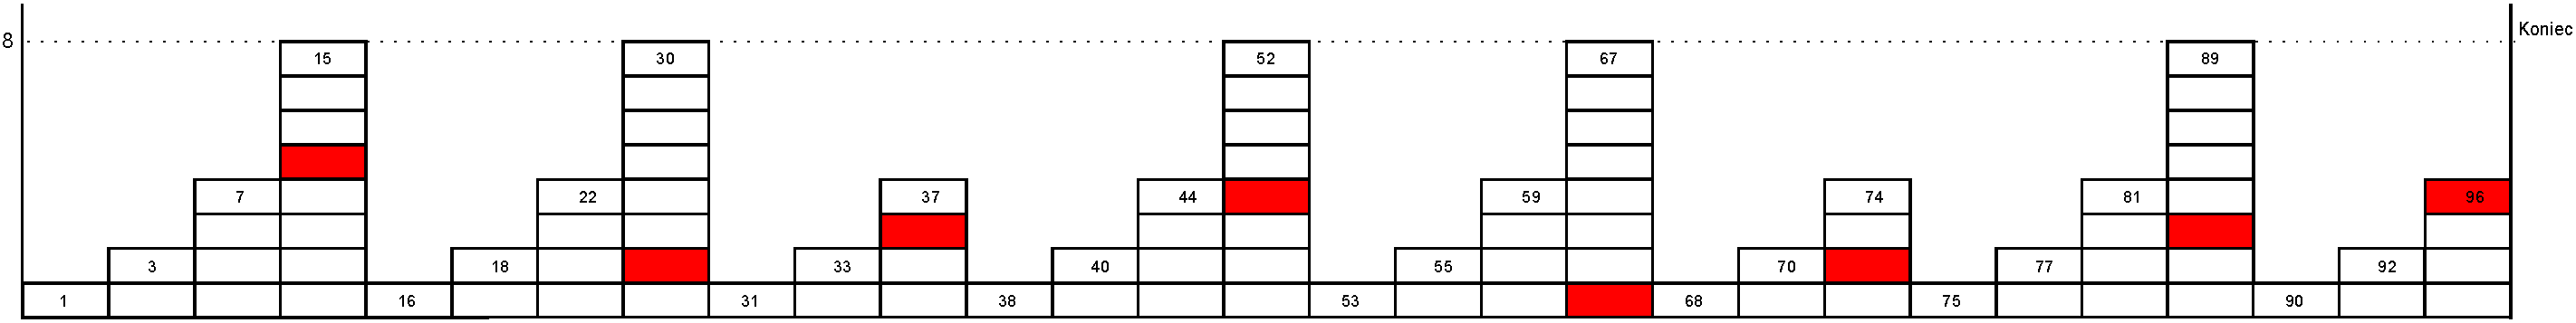
\includegraphics[width=16.0cm]{./images/zadanie08.pdf}\\\\
			Na 96 pakietów 8 zostaje przekłamanych.\\
			Możemy wyróżnić dwa parametry spełniające zadanie:
			\begin{enumerate}
				\item $$ SRET=\frac{(96-8)\cdot 768\;[B]}{29\cdot 45\;[ms]}=\frac{88\cdot 768\;[B]}{29\cdot 45\;[ms]} $$
				\item $$ GBN=\frac{(96-36)\cdot 768\;[B]}{29\cdot 45\;[ms]}=\frac{60\cdot 768\;[B]}{29\cdot 45\;[ms]} $$
			\end{enumerate}
			\small{ \emph{Forczu: w tego typu zadaniach przepustowość chyba zawsze jest maksymalna, a protokoół standardowy, co ma upraszczać całość.
			Ktoś tam napisał, że wielkość ramki we wzorach jest obojętna, ale należy zaznaczyć, czy bierzemy dane czy dane + narzut.}}.
\newpage
	% ================= ZADANIE 5.3 ==================
	\subsection{Zadanie}
		\subsubsection{Treść}
			Stacja robocza podłączona jest z serwerem łączem Fast Ethernet o przepustowości $100\;Mbit/s $, z bitową stopą błędów $ BER=6.6\cdot 10^{-6} $. Uzgodniona wielkość segmentu to 1024 [B] (1088 [B] w łączu), wielkość okna odbiorcy wynosi 27 [kB], czas RTT wynosi 40 [ms]. Określić, ile czasu zajmie przesył 1 [MB] tym łączem protokołu TCP w wersji standardowej.
		\subsubsection{Odpowiedź}
		\begin{enumerate}
			\item $ \cfrac{1}{BER}=\cfrac{1}{6.6\cdot 10^{-6}}=151515$, co oznacza, że 1 na 151515 bitów jest przekłamany $ \rightarrow $ 1 na 18939 bajtów.
			\item $ \cfrac{18939\;[B]}{1\:088\;[B]}\approx17.41 \rightarrow $ co 18 ramka jest przekłamana.
			\item $ \cfrac{27\;[kB]}{1\:088\;[B]}=\cfrac{27\:000\;[B]}{1088\;[B]}=24.82 \rightarrow $, co oznacza maksymalnie 24 ramki w słupku.
			\item
				\begin{center}
					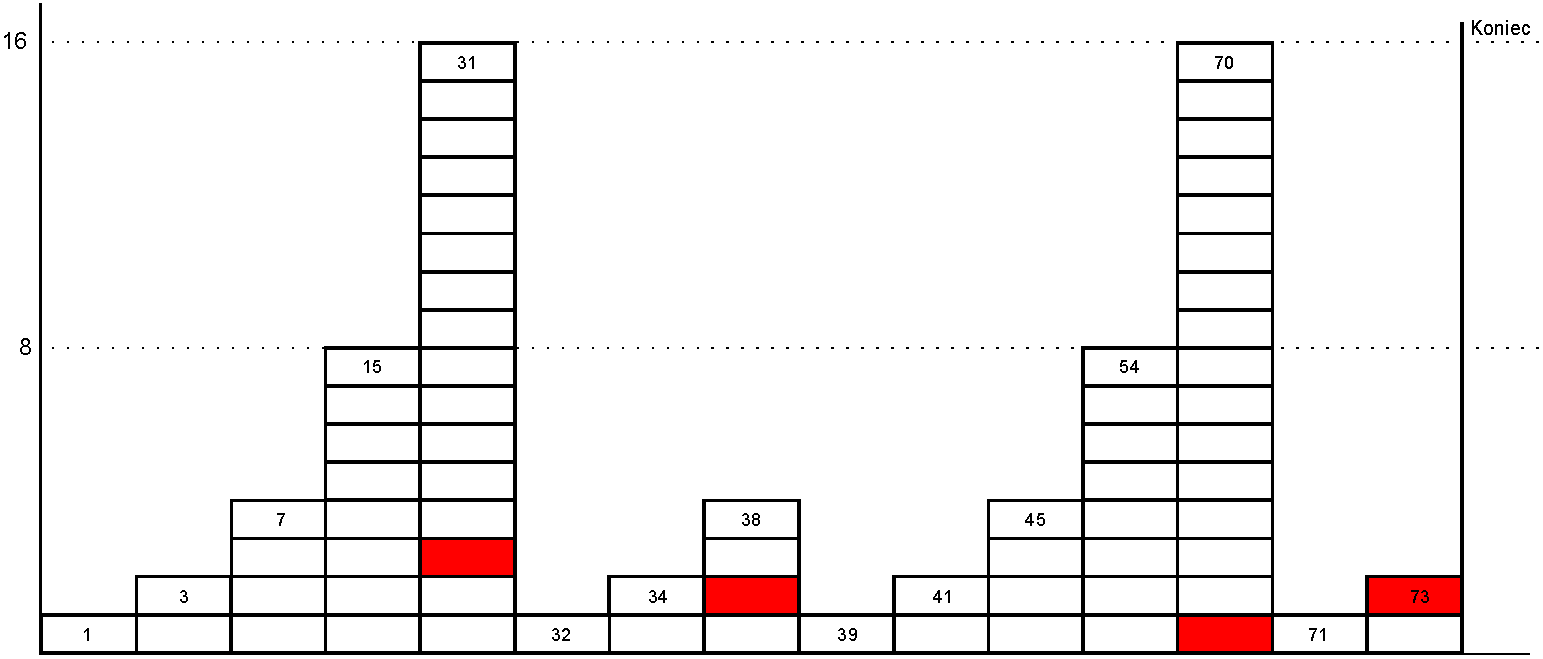
\includegraphics[width=9.0cm]{./images/zadanie14.pdf}
				\end{center}
			\item Odpowiedź
			$$ SRET=\cfrac{68\cdot1024\:[B]}{15\cdot40\:[ms]}\approx113\;[\cfrac{kB}{s}]$$
			$$\\\\ GNB=\cfrac{38\cdot1024\:[B]}{15\cdot40\:[ms]}\approx63\;[\cfrac{kB}{s}]$$
			\item Czas przesyłu 1 MB:\\
			$$ 1024\:[kB] : 113\;[\cfrac{kB}{s}]\approx9.06\;[s] $$\\\\
			$$ 1024\:[kB] : 63\;[\cfrac{kB}{s}]\approx16.25\;[s] $$
		\end{enumerate}
	% ================= ZADANIE 5.4 ==================
\newpage
	\subsection{Zadanie}
		\subsubsection{Treść}
			Użytkownik połączony jest z routerem łączem sieci lokalnej 10 Mbps Ethernet, czas RTT = 35 ms, router dostępowy na obsługę użytkownika przeznacza bufor 12 kB, rozmiar okna protokołu TCP = 27 kB. Określić maksymalną średnią szybkość transmisji możliwą do uzyskania przez użytkownika przez standardowej wersji protokołu TCP.
		\subsubsection{Odpowiedź}
			{\small \emph{Forczu: ponieważ w treści zadania jest podane, że mamy do czynienia z użytkownikiem łączącej się przez router z Internetem to WYDAJE MI SIĘ, że należy wykorzystać algorytm \emph{congestion avoidance}, który ma zastosowanie m.in. w przeglądarkach internetowych. Stąd ta różnica.}}\\
			\begin{enumerate}
				\item Ramka w Ethernecie: 1500 [B] (1460 [B] dla danych)
				\item W routerze jest dostępne 12000 [B].
				\item $ \cfrac{12\:000\;[B]}{1500\;[B]}=8 \rightarrow $ oznacza, że razem można wysłać 8 ramek, przy 9tej przepełni się bufor.
				\item 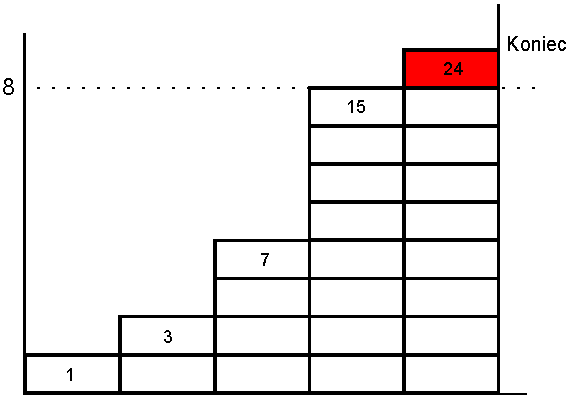
\includegraphics[width=8.0cm]{./images/zadanie15.pdf}
				\item Na 24 ramki 1 została przekłamana. mamy więc 23 poprawne ramki oraz 5 słupków.
				\item $$ SRET=\cfrac{23\cdot1460\:[B]}{5\cdot35\:[ms]}=\cfrac{33580000\:[B]}{175\:[s]}=191885\:[\cfrac{B}{s}]=187\;[\cfrac{kB}{s}] $$
			\end{enumerate}
			
\newpage
% ================= ZADANIE 5.5 ==================
	\subsection{Zadanie}
		\subsubsection{Treść}	
			Stacja robocza jest połączona z serwerem z prędkością 11 [Mbps] i stopą błędów BER = $ 7.3 \cdot 10 ^ {-6} $. Oblicz z jaką średnią prędkością mogą być wysyłane informacje z serwera używając wersji standardowej (\emph{plain vanilla}, \emph{Go Back N}) protokołu TCP. Wynegocjowany segment danych to 768 [B] (ramka w łączu 832 [B]), rozmiar okna to 18.5 [KB], a średni czas RTT to 55 [ms].
		\subsubsection{Odpowiedź}
			\begin{enumerate}
				\item BER = $ 7.3 \cdot 10 ^ {-6} \rightarrow\approx 136986.30\;[b] \approx 17123.29\;[B] $
				\item $ \cfrac{17123.29\;[B]}{832\;[B]}=20.58 \rightarrow $ co 21 ramka przekłamana.\\
				Ponieważ łączem przesyłamy pełne ramki, więc przekłamanie to dane + wszystkie śmiecie.
				\item $ \cfrac{18.5\;[KB]}{832\;[B]}=\cfrac{18\:944\;[B]}{832\;[B]}\approx22.77 $\\
				Oznacza, że SST1 = 23.
			\end{enumerate}
			
			
			
\newpage
	% ================= ZADANIE 5.5 ==================
	\subsection{Zadanie}
		\subsubsection{Treść}
			W systemie transmisji posługującym się protokołem SDLC / HDLC (tryb NRM, w=3, retransmisja grupowa) w łączu ze stopą błędów $ p=10^{-4} $ przesyłane są dane ramkami z polem danych 256 B, ze stacji nadrzędnej do stacji podrzędnej. Przedstaw przebieg transmisji w przesyle \textbf{4.5 kB} danych, pomiń nawiązanie / zrywanie połączenia. Ile kosztuje (narzut protokołu) obsługa błędów w transmisji?
		\subsubsection{Odpowiedź}
			Najpierw liczymy ilość potrzebnych ramek
			$$ \cfrac{4.5\;[kB]}{256\;[B]}=\cfrac{4\:500\;[B]}{256\;[B]}\approx17.58\;[ramek] $$Należy przesłać 18 ramek.\\
			Następnie należy wyliczyć, co którą ramkę pojawi się przekłamanie. Stopa błędu wynosi 1/10000, czyli to oznacza, że co 10000 bit następuje przekłamanie, co równa się 1250 B. Teraz należy obliczyć, co którą ramkę następuje błąd (i teraz nie jestem pewien ale chyba do tych 256 B danych należy dodać 6B nagłówka).
			$$ \cfrac{1250}{262}={4.77}\approx5 $$
			Co piąta ramka zawiera przekłamanie. Teraz można zacząć przedstawiać przebieg transmisji. "w" oznacza ile ramek możemy przesłać w takiej jednej sekwencji.
			\begin{center}
				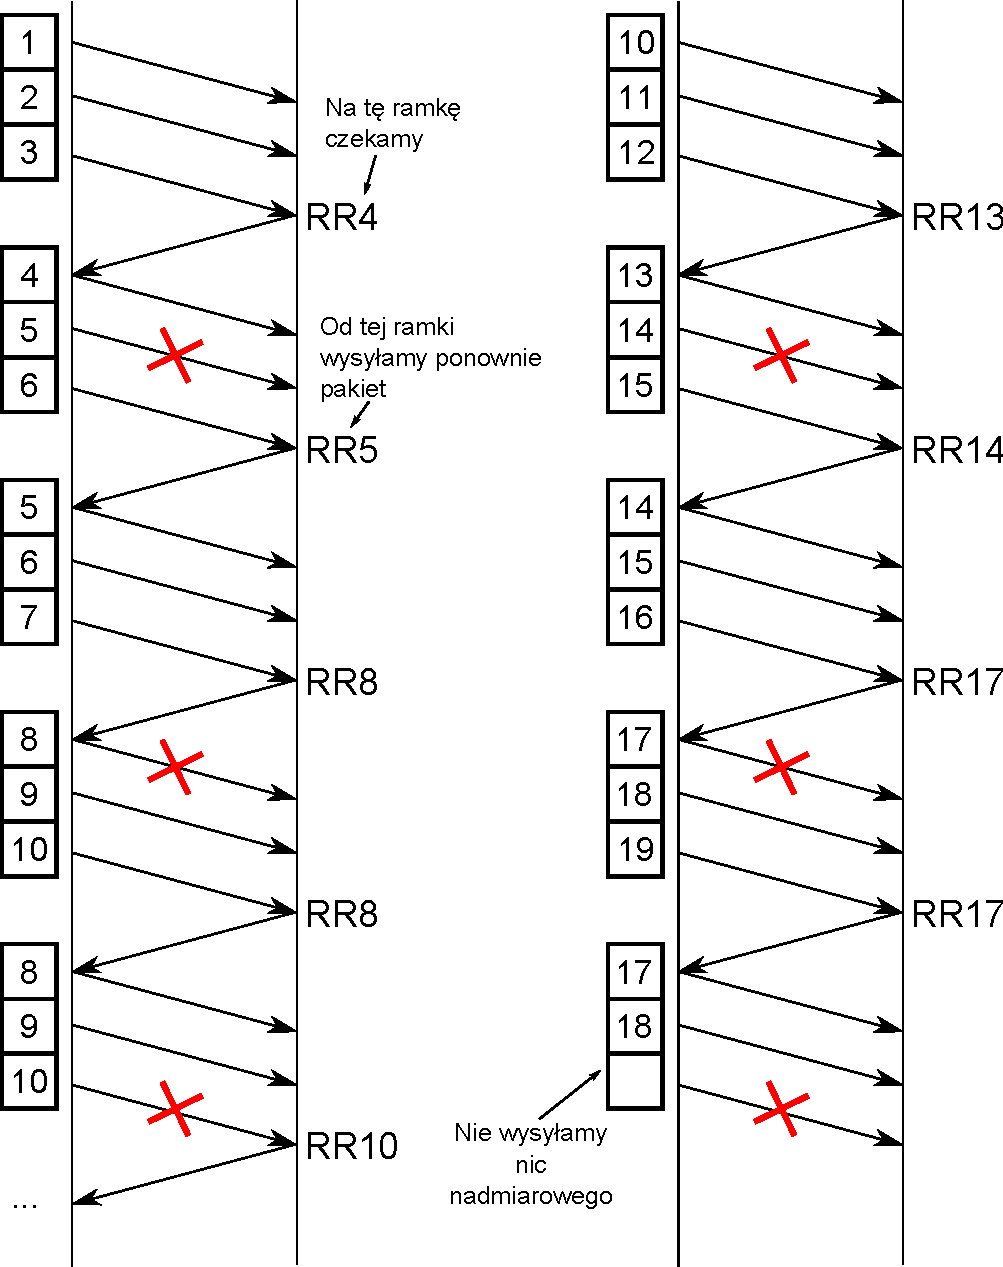
\includegraphics[width=9.0cm]{./images/zadanie09.pdf}
			\end{center}
			Następnie należy policzyć narzut (ilość wszystkich ramek - ilość wymaganych ramek)\\
			$$ Narzut = 28 - 18  = 10\;ramek = 10 * 256\;B = 2560\;B =2,5\; [kB] $$
			\small{ \emph{Forczu: ocenione na 1.0 / 1.0}}.

\newpage
	% ================= ZADANIE 5.6 ==================
	\subsection{Zadanie}
		\subsubsection{Treść}
			W systemie z protokołem SDLC (tryb NRM, w=3, retransmisja grupowa), ze stopą błędów $ p=10^{-4} $, ramki są wysyłane z polem danych 256 B ze stacji nadrzędnej do podrzędnej. Przedstaw przebieg transmisji przy przesyle \textbf{4 kB} danych. Pomiń nawiązanie i zerwanie połączenia. Ile kosztuje (narzut protokołu) obsługa błędów w transmisji?
		\subsubsection{Odpowiedź}
			$ BER=p=10^{-4} \rightarrow$ 1 błąd co 10 000 bitów $ \rightarrow $ 1 błąd do 1250 bajów $ \rightarrow $ 1 błąd w przybliżeniu co 5 ramek.\\
			$$ \cfrac{4\;[kB]}{256\;[B]}=16\;[ramek] $$
			\begin{center}
				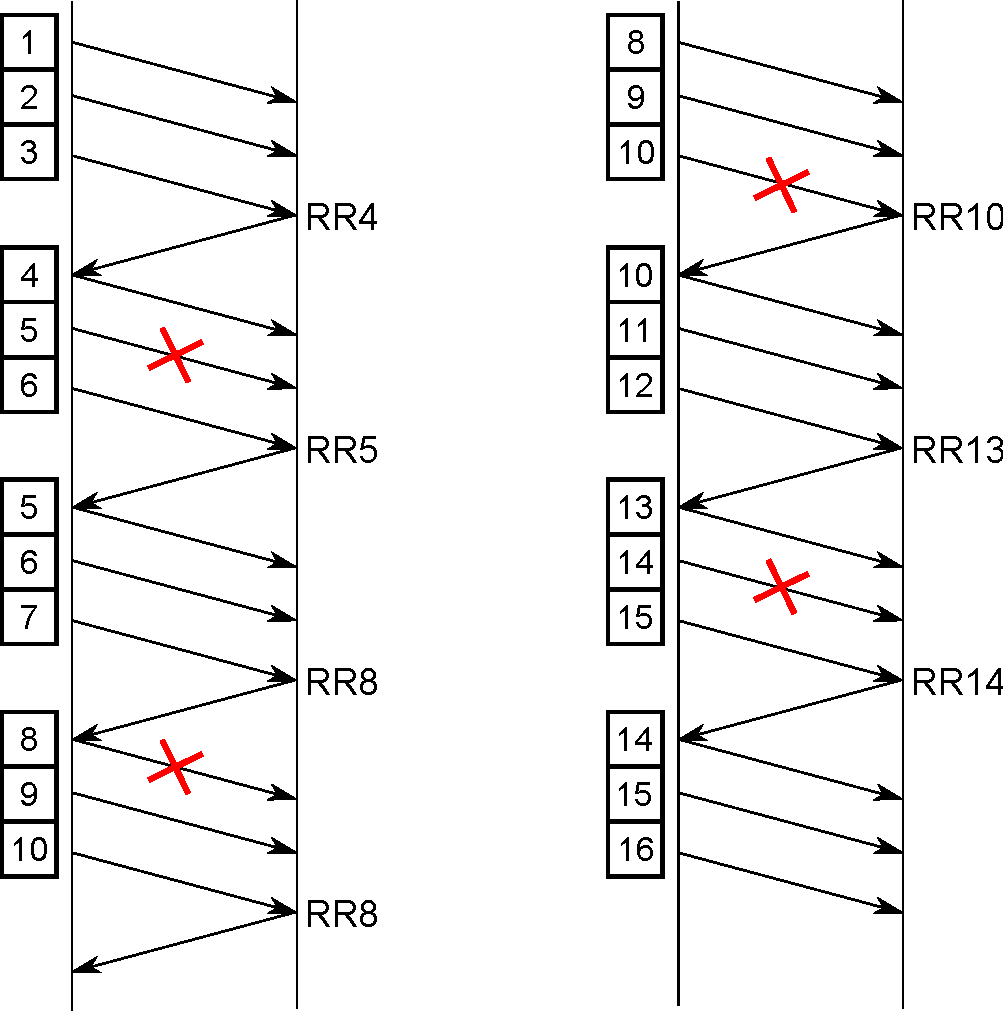
\includegraphics[width=8.0cm]{./images/zadanie10.pdf}
			\end{center}
			Wysłaliśmy łącznie 24 ramki. Narzut: 24 - 16 = 8 ramek = 2048 B = 2 kB
\newpage
	% ================= ZADANIE 5.7 ==================
	\subsection{Zadanie}
		\subsubsection{Treść}
			W systemie transmisji z protokołem HDLC średnio jeden na 9000 bitów jest przekłamany. Jaki będzie koszt obsługi błędów transmisji przy przesyle bloku 4 kB danych ze stacji B do stacji A w tym systemie, jeśli wielkość pola danych to 256 B, okno w=4, tryb NRM z retransmisją grupową.
		\subsubsection{Odpowiedź}
			$$ \cfrac{4\;[kB]}{256\;[B]}=16\;[ramek] $$
			Musimy przesłać 16 ramek.\\
			$ \cfrac{1}{9000} $ bitów przekłamanych $ \rightarrow \cfrac{1}{1125}\;[B] \rightarrow $ co 5 ramka przekłamana.\\\\
			\begin{center}
				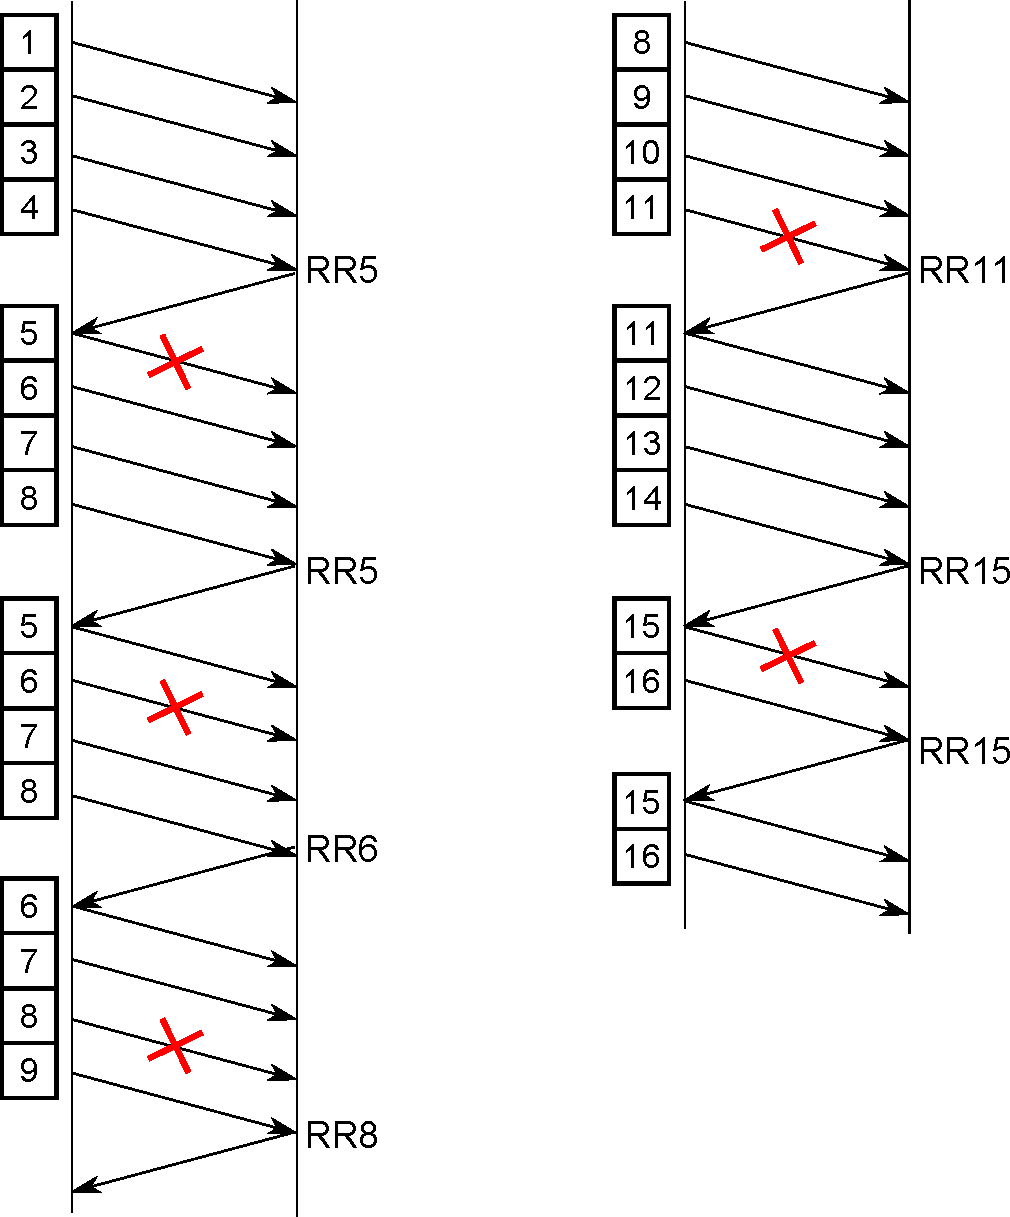
\includegraphics[width=8.0cm]{./images/zadanie12.pdf}
			\end{center}
			Wysłano 28 ramek. Narzut: 28 - 16 = 12 ramek = 3072 B = 3 kB.
\newpage		
	% ================= ZADANIE 5.8 ==================
	\subsection{Zadanie}
		\subsubsection{Treść}
			Drukarka wierszowa posiada jeden bufor na 80 znaków (1 wiersz tekstu). Wydruk bufora zajmuje 25 ms, w czasie których drukarka nie przyjmuje danych. Stacja nadrzędna przesyła notatkę - 3 wiesze (bloki po 80 znaków) łączem o szybkości transmisji 19200 bitów / s, protokół BSC (2 znaki SYN). Przedstaw przebieg komunikacji SN-SP (drukarka). Załóż brak przekłamań, pomiń fazę nawiązania połączenia. Przyjmij czas przetwarzania żądania / odpowiedzi i propagacji sygnału łączem 2.5 $ \mu s $.
		\subsubsection{Odpowiedź}
		Jak mamy bufor to liczymy wg \emph{congestion avoidance}
			19200 $ [\cfrac{b}{s}] $ = 2400 $ [\cfrac{B}{s}] $, czyli 2.4k $ \cfrac{znakow}{s} $, ostatecznie ok. 0.4 ms na jeden znak.
			\begin{center}
				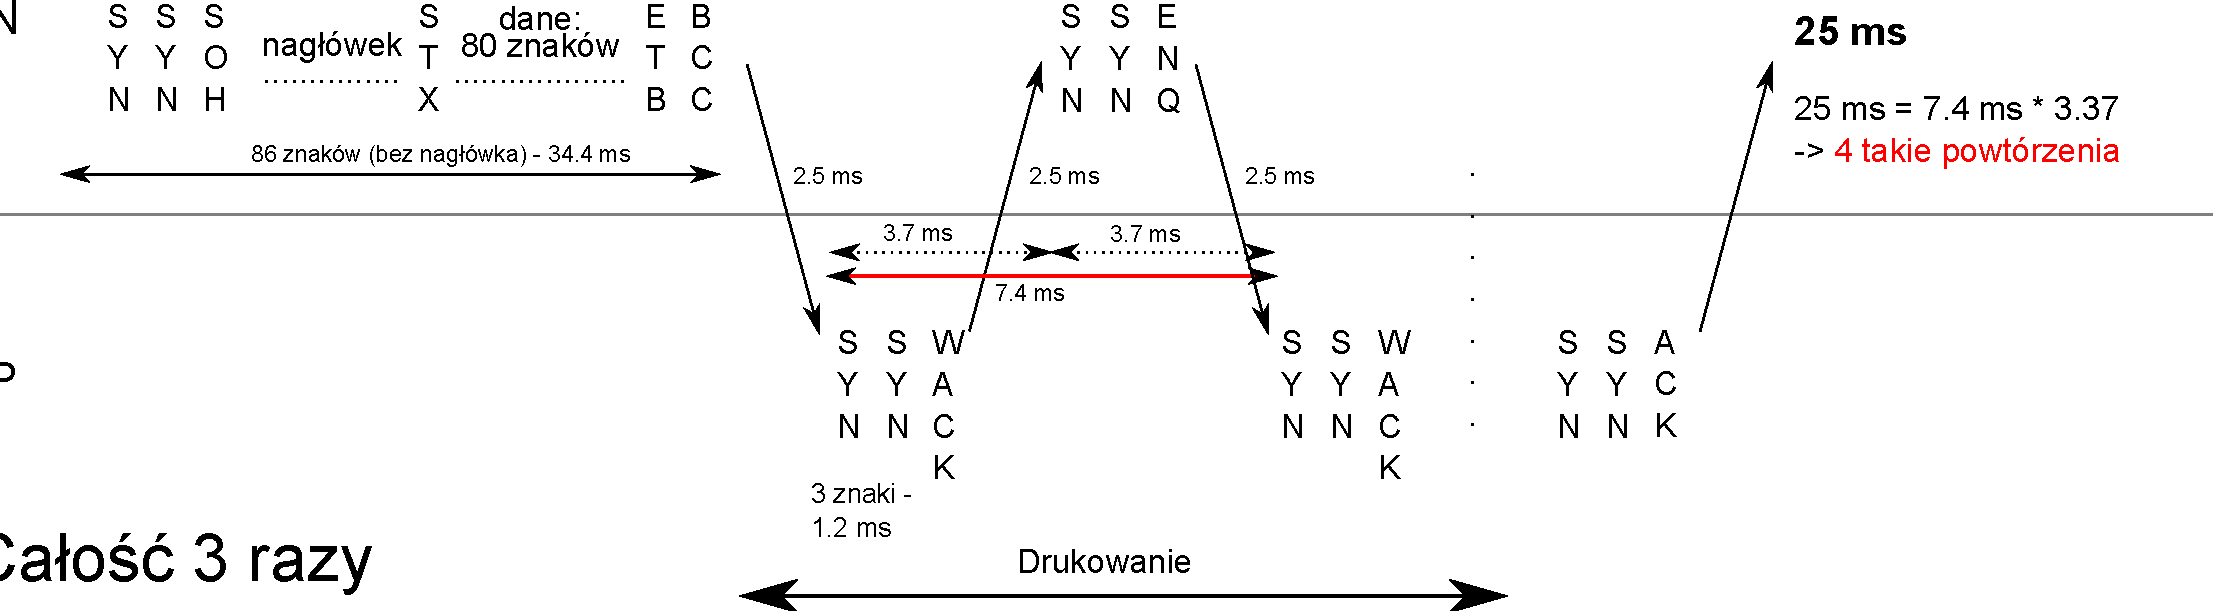
\includegraphics[width=16.0cm]{./images/zadanie13.pdf}
			\end{center}
			\begin{itemize}
				\item Sprowadzamy prędkość transmisji do czasu przesyłu jednego znaku: 1 znak / 0.4 ms. Jest to podstawa do większości czasów.
				\item Stacja nadrzędna, jak się połączy, zaczyna nadawać. Przesyłamy 80 znaków oraz 6 rozkazów. Drukarka odbiera i zaczyna drukować.
				\item Drukowanie ma trwać (minimum) 25 ms. W tym czasie drukarka wysyła WACKi - SN nie wysyła danych, ale zostaje utrzymana komunikacja. SN następnie wysyła zapytania ENQ - czy może przesłać następny wiersz.
				\item Drukarka kończy działanie po 4 wymianach jałowej informacji, po czym wysyła SYN SYN ACK. Po tym sygnale komputer może wysłać kolejne 80 znaków do drukarki. Aby wysłać kolejne 2 wiersze należy całość powtórzyć jeszcze 2 razy.
				\item Podobno swetrowi chodziło bardziej o zilustrowanie procesu niż wyliczania czasów.
			\end{itemize}
			
			
% ==================================================
% --- 6. ADRESACJA
% ==================================================
\newpage
\section{Adresacja}
	% ================= ZADANIE 6.1 ==================
	\subsection{Zadanie}
		\subsubsection{Treść}
			Jak przebiega (po raz pierwszy w danych środowisku) proces tłumaczenia nazwy na adres IP dla nazwy daisy.sales.euro.hp.com? Czy zwracany wynik i proces tłumaczenia różni się czymś przy drugiej próbie w stosunku do pierwszej (odstęp między żądaniami kilka minut, pierwsza zakończona pomyślnie)? Jak będzie przebiegał późniejszy o kilka minut proces tłumaczenia nazwy dino.support.americas.hp.com?
		\subsubsection{Odpowiedź}
			\begin{enumerate}[A]
				\item 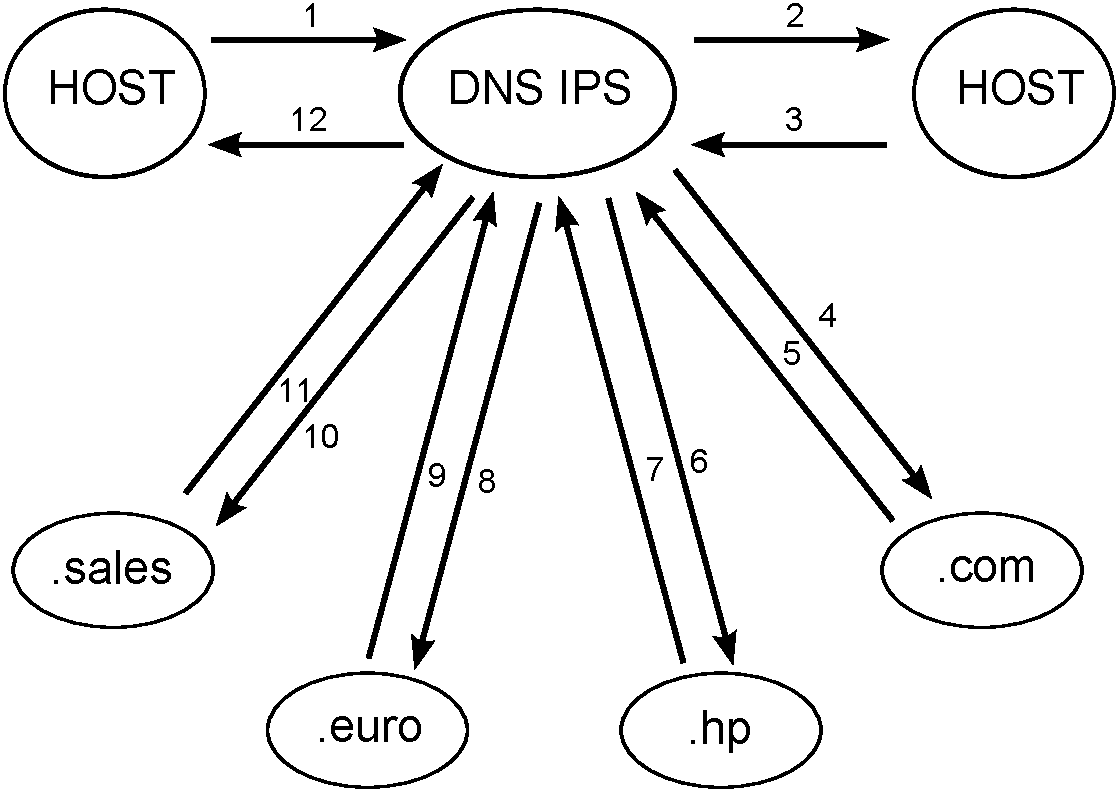
\includegraphics[width=6cm]{./images/zadanie01.pdf}\\
				\begin{enumerate}[1]
					\item Zapytanie DNS o adres IP dla daisy.sales...
					\item Jeśli DNS nie posiada tego adresu to pyta root server
					\item Ten odpowiada, że nie zna adresu IP dla daisy.sales.euro.hp.com , ale zna adres dla com i ... (przekierowuje)
					\item DNS ISP pyta dns com o daisy.sales.euro.hp.com
					\item Ten odpowiada, że go nie zna, ale zna adres dla hp
					\item DNS ISP pyta dns hp o daisy.sales.euro.hp.com
					\item Ten odpowiada, że go nie zna, ale zna adres dla euro
					\item DNS ISP pyta dns euro o daisy.sales.euro.hp.com
					\item Ten odpowiada, że go nie zna, ale zna adres dla sales
					\item DNS ISP pyta dns sales o daisy.sales.euro.hp.com
					\item Serwer sales zwraca adres IP domeny daisy.sales.euro.hp.com. Następnie DNS ISP p(...) go do hosta.
					\item ...
				\end{enumerate}
				\small{ \emph{Brak pełnej treści, ale ocenione na 1.0 / 1.0}}
				\item
					\begin{enumerate}
						\item daisy.sales.euro.hp.com.root
						\begin{enumerate}[1]
							\item Zapytanie do NS .com czy "zna" .hp
							\item Zapytanie do NS .hp czy zna .euro
							\item Zapytanie do NS .euro czy zna .sales
							\item Zapytanie do NS .sales czy zna .daisy
							\item Otrzymanie adresu IP
						\end{enumerate}
						W drugim przypadku adres hp.com może nie być tłumaczony.
						\item dino.support.americas.hp.com
						\begin{enumerate}[1]
							\item Znamy IP (hp.com), pytamy czy zna .americas
							\item Zapytanie do NS czy zna .support
							\item Zapytanie do NS czy zna .dino
							\item Otrzymanie adresu IP
						\end{enumerate}
					\end{enumerate}
					\small{ \emph{Ocenione na 1.0 / 1.0}}
			\end{enumerate}
	% ================= ZADANIE 6.2 ==================
	\subsection{Zadanie}
		\subsubsection{Treść}
			Dostępna jest pewna ilość kolejnych adresów internetowych, zaczynając od 192.170.0.0. Cztery organizacje A, B, C i D występowały kolejno o przydział puli 1000, 2000, 4000 i 1000 adresów IP. Podaj dla każdej z nich pierwszy i ostatni przyznany adres oraz maskę sieci w notacji w.x.y.z i /m.
		\subsubsection{Odpowiedź}
			W treści zadania jest podane, że te firmy przychodziły \textit{kolejno}, więc po prostu w tej kolejności przyznajemy im adresy.
			\begin{enumerate}
				\item Firma A, 1000 adresów - maska na 1024 adresy (niezbędne minimum), czyli odcinamy 10 bitów by utworzyć maskę:
				$$ 11111111.11111111.11111100.00000000=/22=255.255.252.0$$
				\begin{itemize}
					\item Pierwszy adres: 192.170.0.0
					\item Ostatni adres: 192.170.3.255
					\item w.x.y.z: 255.255.252.0
					\item Maska: /22
				\end{itemize}
				\item Firma B, 2000 adresów - maska na 2048 adresy.
				$$ 11111111.11111111.11111000.00000000=/21=255.255.248.0$$
				\begin{itemize}
					\item Nie możemy w połowie wstawić takiej maski, ponieważ wcześniej utworzyliśmy podsieć na 1024 adresy. Dlatego wymagana jest przerwa do uzupełnienia do 2048. Innymi słowy musimy zostawić przerwę po pierwszej podsieci o długości 1024 adresy, by wyrównać je.
					\item Pierwszy adres: 192.170.8.0
					\item Ostatni adres: 192.170.15.255
					\item w.x.y.z: 255.255.248.0
					\item Maska: /21
				\end{itemize}
				\item Firma C, 4000 adresów - maska na 4096 adresy.
				$$ 11111111.11111111.11110000.00000000=/20=255.255.240.0$$
				\begin{itemize}
					\item Tutaj nie musimy dokonywać analogicznego uzupełnienia. W dwóch poprzednich procesach łącznie przeszliśmy przez 4096 adresów, więc tę sieć możemy wstawić bezpośrednio za drugą.
					\item Pierwszy adres: 192.170.16.0
					\item Ostatni adres: 192.170.31.255
					\item w.x.y.z: 255.255.240.0
					\item Maska: /20
				\end{itemize}
				\item Firma D, 1000 adresów - maska na 1024 adresy
				\begin{itemize}
					\item Mamy wolne miejsce między podsieciami dla firmy A i B, tam dajemy tę sieć.
					\item Pierwszy adres: 192.170.4.0
					\item Ostatni adres: 192.170.7.255
					\item w.x.y.z: 255.255.252.0
					\item Maska: /22
				\end{itemize}
			\end{enumerate}
\newpage
	% ================= ZADANIE 6.3 ==================
	\subsection{Zadanie}
		\subsubsection{Treść}
			Firma dysponuje pulą 32 adresów IP. Przyjęto, że pierwszy i ostatni użyteczny adres zostaną przydzielone routerowi dostępowemu i serverowi DNS. Jeden z komputerów otrzymał adres 172.19.21.137. Podaj elementy konfiguracji IP tego komputera.
		\subsubsection{Odpowiedź}
			\begin{itemize}
				\item \textbf{Maska podsieci}: 255.255.255.224 (albo /27)\\
				Firma posiada 32 adresy, które różnią się 5 najmłodszymi bitami. 32 - 5 = 27.
				\item \textbf{Adres IP}: 172.19.21.137
				\item \textbf{Host}: 172.19.21.128 /27 (adres sieci)\\
				Adresem sieci wyliczamy zerując 5 ostatnich bitów. (albo ANDując adres z 1.1.1.11100000)
				\item \textbf{Brama / Router}: 172.19.21.129\\
				Adres routera dostępowego, pierwszy użyteczny adres (00001).
				\item \textbf{Serwer DNS}: 172.19.21.158\\
				Ostatni użyteczny adres (11110). (Broadcast - 1)
				\item \textbf{Broadcast}: 172.19.21.159\\
				Adres rozgłoszeniowy, uzyskany przez "zajedynkowanie" 5 ostatnich bitów. Największy adres w sieci.
				\item Adresy przydzielamy wg kolejnych potęg dwójki $ 2^n $. Gdyby w treści były 33 adresy, to przydzielalibyśmy 64.
				\item Gdyby w treści należałoby podpiąć 32 klientów, to musielibyśmy mieć 34 adresy i znów przydzielać 64.
			\end{itemize}
	% ================= ZADANIE 6.4 ==================
	\subsection{Zadanie}
		\subsubsection{Treść}
			Rekord SOA domeny abc.com zawiera następujące wartości:
			\begin{itemize}
				\item refresh = 10800
				\item retry = 5400
				\item expire = 86400
				\item default TTL = 7200
			\end{itemize}
			Administrator domeny zaplanował zastąpienie wysłużonego głównego \emph{name servera} nowym systemem (nowy adres IP). Po jakim czasie (od dokonania zmiany rekordu NS) równoległej pracy obu \emph{name serverów} będzie można wyłączyć stary serwer.
		\subsubsection{Odpowiedź}	
			Po czasie TTL + refresh = 10 800 + 7200 = 18 000. Gdyby się składało z primary i secondary.
	% ================= ZADANIE 6.5 ==================
	\subsection{Zadanie}
		\subsubsection{Treść}
			Przedstaw jak przebiega proces tłumaczenia adresu IP na nazwę DNS. Jakie domeny TLD są w tym procesie zaangażowane. Ile czasu może maksymalnie zająć przetłumaczenie wcześniej nie znanego adresu, jeżeli odwiedź z NS następują w czasie nie dłuższym niż 0,7s.
		\subsubsection{Odpowiedź}
			Przykładowy adres: 137.57.25.13\\
			Tłumaczenie: 13.25.57.137
			\begin{enumerate}
				\item NS(137) $ \rightarrow $ zapytanie o główny serwer
				\item NS(137.57) $ \rightarrow $ zapytanie o port sieci
				\item NS(137.57.25) $ \rightarrow $ zapytanie o podsieć
				\item NS(137.57.25.13) $ \rightarrow $ zapytanie o nazwę jednostki w swojej podsieci
			\end{enumerate}
			Czas trwania tłumaczenia: $ 4\cdot NS=4\cdot0.7=2.8\:[s] $
			{\small \emph{Forczu: z czyihś notatek.}}
			
% ==================================================
% --- 7. POCZTA E-MAIL
% ==================================================
\newpage
\section{Poczta e-mail}
	% ================= ZADANIE 7.1 ==================
	\subsection{Zadanie}
		\subsubsection{Treść}
			Przedstawić z jakich elementów składa się koperta przesyłki poczty elektronicznej.
			\begin{enumerate}[a)]
				\item Jak przebiega i który z protokołów poczty elektronicznej odpowiada za jej przekazanie?
				\item Jak przebiega odbiór przesyłki przez adresata, który z protokołów obsługuje tę operację?
			\end{enumerate}
		\subsubsection{Odpowiedź}
			\begin{enumerate}[a)]
				\item List elektroniczny wysyłany jest za pomocą protokołu SMTP. Klient inicjuje połączenie poleceniem "helo". Następnie podaje adres nadawcy "mail from", adres odbiorcy "rcpt to", treść listu "data". 
				\\(Koniec części z danymi oznacza pusta linia z '.'. - \textit{doxus}) 
				\\Wiadomość kończy poleceniem "quit".
				\item Listy odbierane są za pomocą protokołów POP3. Klient żąda listy wiadomości poleceniem "list". Następnie pobiera cały żądany list i usuwa go z serwera : "Retr" i "Dele". Sesja kończy się poleceniem "quit". Oczywiście zanim to wszystko nastąpi musi zostać przeprowadzona autentyfikacja. Klient POP3 zaczyna sesję od podania nazwy użytkownika "user" i hasła "pass".
			\end{enumerate}
			\small{ \emph{Ocenione na 1.0 / 1.0}}
	
	% ================= ZADANIE 7.2 ==================
	\subsection{Zadanie}
		\subsubsection{Treść}
			Przesyłka e-mail zawiera fragment tekstu: "płoną góry, płoną lasy..." . Przedstaw sposób zakodowania pierwszych słów treści listu zapewniający (dowolnym łączem) poprawny przesył znaków narodowych.
		\subsubsection{Odpowiedź}
			Zastosowany algorytm to QPE (\emph{Quoted Printable Encoding}). Treść wiadomości:
			\begin{center}
				p\textbf{=B3}on=B9 g\textbf{=F3}ry, p\textbf{=B3}on\textbf{=B9} lasy
			\end{center}
			Gdzie:
			\begin{itemize}
				\item =B3 - dziesiętnie 179 - ł w ASCII
				\item =B9 - dziesiętnie 185 - ą w ASCII
				\item =F3 - dziesiętnie 243 - ó w ASCII
			\end{itemize}
			Dziesiętne kody w ASCII były podane w poleceniu, należało je zmienić na zapis szesnastkowy.	
\newpage
	% ================= ZADANIE 7.2 ==================
	\subsection{Zadanie}
		\subsubsection{Treść}
			Tekst w języku polskim zawiera średnio 5\% znaków narodowych. Porównać efektywność kodowania (zwiększenie objętości) przesyłek e-mailowych dla obu (dostępnych w MIME) metod bezpiecznego przesyłu rozszerzonego zestawu znaków ASCI. Przy jakim procencie znaków narodowych w przesyłanym tekście efektywność obu metod będzie taka sama?
		\subsubsection{Odpowiedź}
			1 znak polski = 3 znaki dla QP.\\
			Np. 5\% polskich znaków - na 100 znaków przypada 5 polskich. Zostanie wysłanych 110 znaków - nadmiarowość QP wynosi 10\%.\\
			Dostępne rozwiązania:
			\begin{enumerate}
				\item Queted Printable - nadmiarowość 10\%
				\item Base64 - nadmiarowość 33\%
			\end{enumerate}
			Oznacza to, że dla 5\% znaków obie metody będą miały równą sprawność przy
			$$ \cfrac{10}{100}\cdot5=\cfrac{33}{100}\cdot x \rightarrow x = \cfrac{10}{100}\cdot\cfrac{100}{33}\cdot 5 = 16.5 $$
			znakach.
			
% ======================================================
% --- 8. INNE
% ======================================================
\newpage
% ================= ZADANIE 8.1 ==================
\section{Inne}
	\subsection{Zadanie}
		\subsubsection{Treść}
			Posłaniec przewozi nagrane płyty DVD (9 GB informacji) poruszając się ze średnią szybkością 60 km/h. Do jakiej odległości ma on szybkość przesyłu większą niż sieć 10 Mbitów/s.
		\subsubsection{Odpowiedź}
			$$ 60\:[\cfrac{km}{h}]=\cfrac{60\:000 [m]}{3600\:[s]}=16\frac{2}{3} [\frac{m}{s}] $$
			$$ 6\:[GB] / 10\:[MBit/s] = \cfrac{768\:[Mbit]}{10\:[MBit/s]}=76.8\:[s]$$
			$$ 16\frac{2}{3} [\frac{m}{s}] \cdot 76.8\:[s] \approx 1280.256 $$
			
			